%%\documentclass[usenatbib,usegraphicx,letterpaper]{mnras}
\documentclass[usenatbib,fleqn]{mnras}
\pdfoutput=1 %for arxiv
\setlength{\topmargin}{-0.3in}
%%\usepackage[totalwidth=480pt,totalheight=680pt]{geometry}
\usepackage{amssymb}
\usepackage{epsfig}
\usepackage{amsmath}
\usepackage{color}
\usepackage[dvipsnames]{xcolor}
\usepackage{epsfig}  
\usepackage{graphicx}
\usepackage{subfig}
\usepackage{rotating}
\usepackage{fixltx2e}
\usepackage[T1]{fontenc}
\usepackage{newtxtext,newtxmath}
\usepackage[figure,figure*]{hypcap}
%%\usepackage{physics}

%Journals
\def\pasj{{PASJ}}
\def\nat{{ Nature }}
\def\aap{{ Astron. \& Astrophys. }}
\def\aj{{ Astron.~J. }}
\def\apj{{ Astrophys.~J. }}
\def\araa{{ Ann. Rev. Astron. Astrophys. }}
\def\apjl{{ Astrophys.~J.~Letters }}
\def\apjs{{ Astrophys.~J.~Suppl. }}
\def\apss{{ Astrophys.~Space~Sci. }}
\def\icarus{{ Icarus }}
\def\mnras{{ MNRAS }}
\def\pasp{{ Pub. Astron. Soc. Pacific }}
\def\planss{{ Plan. Space Sci. }}
\def\physrep{{ Phys. Rep.}}
\def\jcap{{J. Cosm. Astropart. Phys.}}

% less then similar, greater than similar
\def\lsim{\lower0.6ex\vbox{\hbox{$ \buildrel{\textstyle <}\over{\sim}\ $}}}
\def\gsim{\lower0.6ex\vbox{\hbox{$ \buildrel{\textstyle >}\over{\sim}\ $}}}

% begin equation
\newcommand{\beq}{\begin{equation}}
\newcommand{\eeq}{\end{equation}}
\newcommand{\beqa}{\begin{eqnarray}}
\newcommand{\eeqa}{\end{eqnarray}}

% basic cosmology
\newcommand{\Ho}{H_{0}}
\newcommand{\Om}{\Omega_{\mathrm{M}}}
\newcommand{\Ol}{\Omega_{\Lambda}}
\newcommand{\Ode}{\Omega_{\mathrm{DE}}}
\newcommand{\rhocrit}{\rho_{\mathrm{crit}}}
\newcommand{\Ok}{\Omega_{\mathrm{K}}}
\newcommand{\wzero}{w_{0}}
\newcommand{\wa}{w_{\mathrm{a}}}
\newcommand{\wpiv}{w_{\mathrm{piv}}}
\newcommand{\apiv}{a_{\mathrm{piv}}}
\newcommand{\ellmax}{\ell_{\mathrm{max}}}
\newcommand{\fsky}{f_{\mathrm{sky}}}

\newcommand{\fom}{\mathcal{F}}
\newcommand{\Rvir}{r_{\mathrm{vir}}}
\newcommand{\Rdel}{r_{\Delta}}

% units
\newcommand{\Msun}{\mathrm{M}_{\odot}~}
\newcommand{\hMsun}{\ h^{-1}\mathrm{M}_{\odot}~}
\newcommand{\hMpc}{\ h^{-1}\mathrm{Mpc}~}
\newcommand{\hkpc}{\ h^{-1}\mathrm{kpc}~}
\newcommand{\cpiv}{c_{\mathrm{piv}}}
\newcommand{\kmsmpc}{~\mathrm{km/s/Mpc}~}
\newcommand{\kms}{~\mathrm{km}~\mathrm{s}^{-1}}
\newcommand{\Mpc}{\mathrm{Mpc}}
\newcommand{\kpc}{\mathrm{kpc}}
\newcommand{\pc}{\mathrm{pc}}
\newcommand{\au}{\mathrm{AU}}
\newcommand{\gev}{\mathrm{GeV}}

% roman differential
%\newcommand{\dd}{\mathrm{d}}

% comments
\newcommand{\arz}[1]{{\color{BrickRed}\textbf{[ARZ: }\textbf{#1}]}}


%%\bibliographystyle{mn2e}
\bibliographystyle{mnras}

%%%%%%%%%%%%%%%%%%%%%%%%%%%%%%%%%%%%%%%%%%%%%%%%

\begin{document}


\title[The Immitigable Nature of Assembly Bias]{The Immitigable Nature of Assembly
Bias: the Impact of Halo Definition on Environmental Effects}
\author[A. Villarreal et al.]{%
Antonio S. Villarreal,$^{1}$\thanks{E-mail: asv13@pitt.edu}
Andrew R. Zentner,$^{1}$\thanks{E-mail: zentner@pitt.edu}
Yao-Yuan Mao,$^{1}$\thanks{E-mail: yymao@pitt.edu}
\newauthor
Christopher W. Purcell,$^{2}$\thanks{E-mail: cwpurcell@mail.wvu.edu}
Andrew P. Hearin,$^{3}$\thanks{E-mail: andrew.hearin@yale.edu}
Frank C. van den Bosch,$^{3}$\thanks{E-mail: frank.vandenbosch@yale.edu}
\newauthor
and Benedikt Diemer$^{4}$\thanks{E-mail: benedikt.diemer@cfa.harvard.edu}
\\
$^{1}$Department of Physics and Astronomy \& Pittsburgh Particle Physics, Astrophysics, and Cosmology Center (Pitt-PACC), \\
\phantom{$^{1}$}University of Pittsburgh, Pittsburgh, PA\\
$^{2}$Department of Physics and Astronomy, West Virginia University, Morgantown, WV \\
$^{3}$Department of Astronomy, Yale University, Hew Haven, CT\\
$^{4}$Center for Astrophysics, Harvard University, Cambridge, MA}

\date{\today}

\pagerange{\pageref{firstpage}--\pageref{lastpage}} \pubyear{2017}

\label{firstpage}

\maketitle

\begin{abstract}
%% Abstract goes here
Recent work has shown the importance of environment to the properties of dark matter halos. This brings conflict
to standard implementations of the halo model and excursion set theory which assume that the properties of a
population within the halo is determined by the mass of the halo alone. We seek to find a definition of the size
of a halo that allows us to minimize the impact of assembly bias on halo model calculations. We analyze the
dependence on environment of our properties using the method of marked correlation functions for several
different halo definitions, utilizing the \citet{diemer_kravtsov15} simulations. We find that the strength of assembly
bias has a strong dependence on the measured halo mass, even when using marks normalized around fixed mass. We note that differences in halo definition, sample selection, and properties of interest can greatly impact
the measurement of assembly bias, potentially explaining conflicting results in the literature. These results suggest that
halo assembly bias appears increasingly difficult to resolve using the definitions common in current halo finder techniques,
possibly pointing toward the necessity of methods such as utilizing the halo splashback radius.
\end{abstract}

\begin{keywords}
cosmology: dark matter -- cosmology: large-scale structure of Universe -- galaxies: formation --galaxies: halos -- methods: numerical
\end{keywords}

%% notes on citation style:
%% \citep{stuff01,stuff02,stuff03} produces (Stuff 2001; Stuff 2002; Stuff 2003)
%% \citet{stuff04} produces "Stuff (2004)" in the main body
%% \\* defines a break in a section title it appears?
%% \begin{enumerate} into \item allows you to do the (i), (ii), (iii) thing 


%-----------------------
\section{Introduction}
\label{section:introduction}
%-----------------------

In the concordance cosmology, galaxies and clusters form within dark matter halos \citep{white_rees78,blumenthal_etal84, mo_etal10}. Numerical simulations have provided a solid understanding of the abundances, properties, and 
clustering of dark matter halos in the standard cosmological model. Accordingly, it is possible to compute the 
clustering statistics of galaxies given a model for the relationship between galaxies and dark matter halos. 
Such halo occupation models have been used to interpret large-scale structure measurements and 
constrain models of galaxy evolution \citep{yang_etal03,tinker_etal05,zehavi_etal05b,porciani_norberg06,vdbosch_etal07,zheng_etal07,conroy_wechsler09,
yang_etal09b,zehavi_etal11,guo_etal11a,wake_etal11,yang_etal11a,yang_etal12,leauthaud_etal12,
rodriguezpuebla_etal12, behroozi_etal13b, moster_etal13, tinker_etal13,cacciato_etal13,more_etal13,guo_etal14,
zu_mandelbaum15b}.
To date, the vast majority of halo occupation models rely on a key assumption, namely that 
the probability of a halo to host a number of galaxies of a particular type 
depends only upon halo mass. It is now well known that the clustering strength of halos depends upon 
properties such as halo formation time \citep{gao_etal05,harker_etal06, wechsler_etal06,gao_white07,croton_etal07,zentner07,dalal_etal08, li_etal08, lacerna_padilla11}, 
concentration \citep{wechsler_etal06,faltenbacher_white10, mao_etal15}, and other halo properties \citep{bett_etal06, hahn_etal07a, hahn_etal07b, faltenbacher_white10, vandaalen_etal12, fisher_faltenbacher16, sunayama_etal16, chavesmontero_etal16}. 
If galaxy properties depend upon these halo properties, a phenomenon known as galaxy {\em assembly bias}, 
then standard halo occupation modeling will fail \citep{zentner_etal14} 
and more complex models \citep{gilmarin_etal11, hearin_etal16} are necessary.


In this work, we explore the possibility of simplifying halo occupation modeling, at least for some 
applications, by altering the definition of a halo. Though motivated broadly by spherical collapse \citep{gunn_gott72, fillmore_goldreich84, ryden_gunn87, lacey_cole93, eke_etal96, mota_vandebruck04, pace_etal10} \arz{Cite the classic spherical collapse 
papers here, such as Lacey \& Cole 1993 and so on.}\asv{Unsure if I missed anything we want to cover in specific.}, specific halo definitions have become a matter of convention that vary considerably in the literature. Many 
authors define halos using a friends-of-friend (FoF) algorithm applied to the particle distribution \citep{davis_etal85, knebe_etal11} \arz{Cite the famous Davis, Efstathiou, Frenk, and White paper from the 1980s}\asv{I think the Knebe et al covers a lot of halo finders, so that should help.}. More often, authors define halos by spherical overdensity (SO) regions within which the mean density exceeds a particular threshold \citep{knebe_etal11}. The threshold used 
varies significantly. With respect to the mean density of the universe, 
commonly used thresholds are 178, 180, 200, and $\sim$340 times the mean 
background density, the last of these being the ``virial" overdensity in a concordance $\Lambda$CDM universe. 
Significantly higher values of the overdensity parameter are often used in studies of X-ray emission from cluster-sized halos.


Our work is an attempt to exploit halo definition to work for the 
convenience of the practitioner. We study the strength of various halo assembly bias signals as a function of halo definition. This is motivated, in large part, by recent literature that suggests 
that a large portion of assembly bias stems from halos in the relatively dense environments surrounding larger halos \citep{wang_etal07, warnick_etal08, more_etal15,sunayama_etal16}. Moreover, 
the environmental impacts of halos on one another has been shown to extend beyond well beyond traditional virial radii. 
\citep{adhikari_etal14, diemer_kravtsov14, wetzel_etal14, more_etal15, wetzel_nagai15} Halos in dense environments (e.g., near other large halos) exhibit anomalous properties 
(e.g., formation times, concentrations, etc.) compared to field halos 
in part because of their interactions with their larger, neighbor halos. It seems interesting to ask 
whether or not a halo definition in which large halos contain many of these smaller, anomalous neighbor halos, thus 
using the halo concept to draw a more meaningful boundary around regions within which highly nonlinear effects are important, can mitigate halo assembly bias. Assessing this strategy is the aim of our paper. 


We restrict ourselves to halos that are defined by spherical regions and we study the strength of halo assembly bias as a function of the density threshold used to demarcate these halos. We find that for halo properties that measure the degree of central mass concentration, there exist halo definitions in which assembly bias may be 
greatly mitigated. However, the definitions which mitigate concentration-based assembly bias are mass dependent; high-mass, cluster-sized halos appear to have little assembly bias 
for a traditional overdensity definition of $\Delta \approx 200$, 
while low-mass halos ($\sim 10^{11}\, h^{-1}\mathrm{M}_{\odot}$) require 
$\Delta \approx 20$. Any mitigation strategy must be complex and mass dependent, as might be expected given the mass dependence of the assembly bias effect \cite{wechsler_etal06}. 
We find that we cannot mitigate the assembly bias of halos selected by properties other than concentration, such as halo spin, halo shape, and number of satellite halos. These results suggest that any mitigation scheme will likely be quite complex if it all practical. \arz{I plan to add something here after I complete my run through the paper.}

 
In \S~\ref{section:data} of this paper, we discuss the cosmological simulations and halo finders
utilized in the analysis. In \S~\ref{section:haloprops}, we discuss 
and define the halo properties used as our tracers of assembly bias. In \S~\ref{section:methodology}, 
we discuss the statistics that we use to measure environmental effects after
halo redefinition. We also discuss our method of removing known mass scaling from halo properties.
In \S~\ref{section:results}, we present our findings and consider how the change
of halo definition impacts measures of assembly bias. In
\S~\ref{section:conclusions}, we discuss the significance of our results in the context of halo modelling.
 We also consider the nature of assembly bias as a function of halo definition.





%------------------------------------
\section[]{Simulations and Halo Identification}
\label{section:data}
%------------------------------------


In order to study the effects of halo redefinition, we use three cosmological $N$-body simulations of structure
formation. The \citet{diemer_kravtsov15} simulations each utilize a Planck best-fit cosmology with $\Om = 0.32$, $\Ol =
0.68$, and $h_0 = 0.67$. We use three simulation boxes with comoving sizes of 125, 250, and 500
$\hMpc$ respectively. The particle masses are $1.6 \times 10^8$, $1.3 \times 10^9$, and $1.0 \times 10^{10}
\hMsun$ respectively, implying a total of $1024^3$ particles in each simulation. The three
simulations have force softening scales of $2.4$, $5.8$, and $14 \hkpc$. We refer to each simulation as
\simA, \simB, or \simC~  for the remainder of the paper. This set of simulations allows us to probe the
resolution effects inherent in halo finding (due to the varying resolutions of the simulations) and to probe the
mass dependence of halo clustering over a wider range of halo masses than would be possible with only one
simulation from the set. For example, \simA, with its higher resolution, contains the least massive resolved
halos, while \simC~has the most robust statistics for the most massive halos as a result of the larger simulation
volume.


To identify halos, we use the {\tt ROCKSTAR} halo finder, which works on the phase space algorithm described in
\citet*{behroozi_etal13a}. In short, {\tt ROCKSTAR} determines initial groupings of particles using a Friends-of-Friends algorithm 
in phase space before applying the spherical overdensity halo definition in order to determine halo properties of
interest. Unbound particles are removed prior to the calculation of halo mass and other halo properties. Our
method of halo redefinition is to change how halo size is calculated as part of the {\tt ROCKSTAR} pipeline. 
A halo is given a radius, $\Rdel$, determined by
\beq
	\bar{\rho}(\Rdel) = \Delta \rho_{\mathrm{m}}, 
\eeq
where the mean density within a spherical volume of radius $r$ is $\bar{\rho}(r)$, $\Delta$ is the overdensity
parameter, and $\rho_{\mathrm{m}}$ is the mean background mass density of the simulation. The resulting
halo size calculation can have a large variation depending on the choice of $\Delta$. The number chosen for
$\Delta$ varies throughout the literature from $\Delta \approx 178$ to $\Delta \approx 340$ or higher for X-ray studies of 
clusters. We choose to vary the size of a halo by treating the overdensity parameter as tunable, expanding the range from 
$\Delta = 340$ to $\Delta = 20$. While this range is greater than the differences between most 
the common overdensity choices, this broad range enables a fairly extensive exploration of 
environmental effects on halo properties as a function of halo definition\footnote{It is worth noting that the 
{\tt ROCKSTAR} linking length parameter must be adjusted as $\Delta$ varies in order to ensure 
that SO halos contain all relevant particles. The value we choose ($0.4 \hMpc$) is large enough that it works for all definitions, but is poorly optimized for speed.}.
\arz{I think that for completeness, you have to quote the 
linking length parameters that you used so that somebody 
else can test your methods if they want to. Please add this.}\asv{Added to the footnote.}

An additional benefit of the {\tt ROCKSTAR} software is the ability to identify substructure, commonly referred to in the
literature as subhalos. Effectively, all density peaks are identified within the simulation and if a halo exists within the phase
space of another halo, the less massive of the two is defined to be a subhalo of the more massive companion. The more massive companion is 
referred to as the host halo. This process continues until all halos identified in the simulation have been designated as either host halos or subhalos.

%-------------------------------------
\section{Halo Properties}
\label{section:haloprops}
%-------------------------------------

As has long been well known, halo mass is the property that most strongly affects halo clustering. In 
this paper, we aim to study the strength of halo clustering as a function of halo properties other than 
mass. We will refer to these properties as ``auxiliary" halo properties in this paper. The properties 
we study are described in this section.

%----------------------------------------
\subsection{Measures of Halo Concentration}

We investigate the clustering of halos as a function of a number of halo properties 
that have been shown to influence halo clustering at fixed halo mass. We explore 
two definitions of halo concentration. The first stems from a fit of the spherically-averaged 
halo density profile, $\rho(r)$, to a \citet{navarro_etal97}; hereafter, NFW density profile, 
%
\beq
\rho(r) = \frac{\rho_0}{\frac{r}{r_{\mathrm{s}}}(1+\frac{r}{r_{\mathrm{s}}})^2},
\eeq
%
where the density scale, $\rho_0$, and the scale radius, $r_{\mathrm{s}}$, are parameters 
that are fit to the density profile of each halo. The standard definition of halo concentration is then 
\beq
c_{\mathrm{NFW}} = \frac{\Rdel}{r_\mathrm{s}},
\eeq
where $\Rdel$ is the radius of the halo given an overdensity parameter, $\Delta$, defining the halo 
and $r_{\mathrm{s}}$ is the inferred halo scale radius. We use the NFW concentrations computed by the 
{\tt ROCKSTAR} halo finder, which are derived from a fit to the halo density profile.  


The NFW concentration defined in the previous paragraph has the shortcoming that it 
depends upon a parametric description of dark matter halos, so we study the clustering dependence 
of halos as a function of a non-parametric description of halo concentration as well. In particular, we 
use the ``velocity-ratio" concentration,
\beq
c_{\mathrm{V}} = \frac{V_{\mathrm{max}}}{V_{\Delta}}, 
\eeq
where $V_{\mathrm{max}}$ is the maximum circular velocity achieved within the halo and $V_{\Delta}$ is 
the circular velocity at the halo radius, $\Rdel$. All halos of the same mass have the same value of $V_{\Delta}$; however, 
they exhibit a variety of $V_{\mathrm{max}}$ values depending upon the degree to which their masses are concentrated toward 
the halo center. The quantity $c_{\mathrm{V}}$ is a non-parametric measure of halo concentration and can be measured from 
simulation snapshots without fitting halo density profiles. Consequently, $c_{\mathrm{V}}$ is robust to halo density 
profile parameterizations and halo profile fitting procedures. 


Halo concentrations are interesting to investigate for these purposes for a number of reasons. 
First of all, the environment dependence of halo concentrations is known to be strong for 
standard halo definitions. Second, halo concentrations are of interest in the modeling of 
galaxy clustering and gravitational lensing statistics (and their cross correlations). 
In the case of galaxy clustering, the relevance is indirect, because galaxies may 
not trace the mass densities of their host halos. In the case 
of gravitational lensing, the mass distribution is the primary quantity of interest and halo concentrations are 
directly related to predictions for lensing statistics. Third, concentrations can be measured from 
individual simulation snapshots easily and halo concentrations are known to be strongly correlated with 
the formation histories of dark matter halos with earlier forming halos having higher concentrations at 
fixed halo mass \citep{wechsler_etal02, zhao_etal03, wechsler_etal06, zhao_etal09}. 
As such, exploring the concentration dependence of halo
clustering may yield insight into the age dependence of halo clustering without the need for constructing merger
trees. This is particularly important in the present study in which the halo finding is performed repeatedly for many 
different values of $\Delta$. Constructing a self-consistent merger tree from which halo formation history can be 
studied requires halo finding at all simulation snapshots for each new value of $\Delta$, which is a computationally 
prohibitive task. 

In the present paper, we limit our study to halo properties that can be measured from a single simulation 
snapshot. However, halo formation histories correlate with halo concentrations with significant scatter and this correlation may 
depend upon environment, so the reader should be wary of drawing conclusions about the environmental dependence of 
halo formation by extrapolating our results on halo concentration. 
We will explore measures of halo age directly in a forthcoming follow-up study dedicated to halo 
formation histories.

Figure~\ref{fig:cnfwrelation} shows the mean $c_{\mathrm{NFW}}$-$M_{\Delta}$ relation for halos defined with
$\Delta=200$ in \simA, \simB, and \simC. For each simulation, we consider halos only above a minimum mass threshold 
to ensure that property measurements are not compromised by resolution effects. The minimum mass 
thresholds are shown as the vertical lines in Fig.~\ref{fig:cnfwrelation} and listed in Table~\ref{table:thresholds}. 
Similar to Fig.~\ref{fig:cnfwrelation}, Figure~\ref{fig:cvrelation} shows the relation between the 
velocity-ratio concentration, $c_{\mathrm{V}}$, and halo mass. 
In the interest of completeness, Figure~\ref{fig:concentrations} shows the relationship 
between $c_{\mathrm{NFW}}$ and $c_{\mathrm{V}}$ on a halo-by-halo basis. As is evident, 
the two concentration proxies are strongly correlated and exhibit a $\sim 6\%$ scatter indicating 
that $c_{\mathrm{NFW}}$ and $c_{\mathrm{V}}$ indeed encode similar information about each 
halo.

%------------------------------------------ Figure for Cnfw(M)
\begin{figure}
\centering
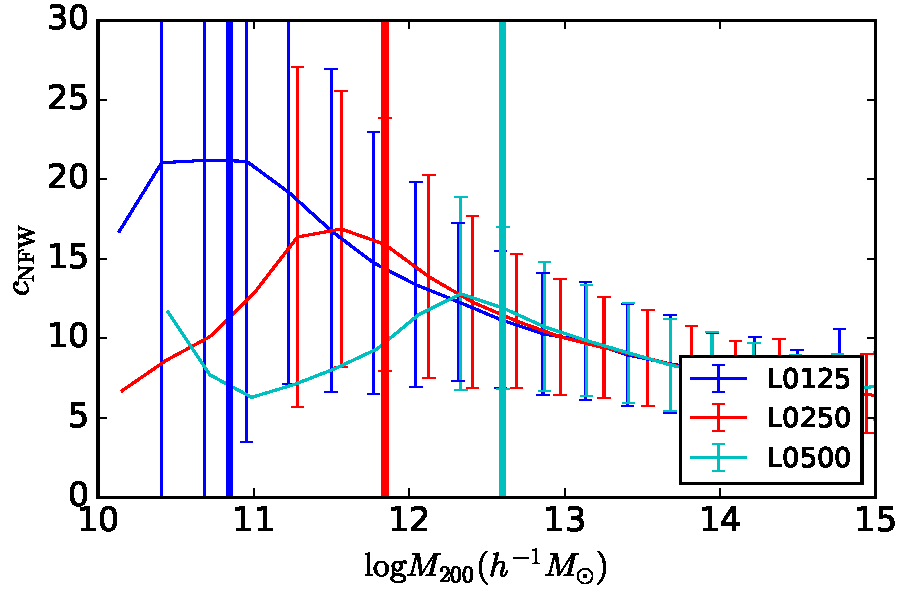
\includegraphics[width=.45\textwidth]{masscut_cNFW_d200.pdf}
\caption{
The relationship between the NFW concentration and halo mass for each of our simulations with $\Delta =200$. 
In order of increasing simulation volume, the blue line corresponds to the concentration-mass relation from simulation 
\simA, the red line corresponds to \simB, and the cyan line corresponds to \simC. The red error bars show the 68\% spread in
parameter values within that mass bin for \simB. These errors are comparable to those of the other simulations
within the region of interest.
Each simulation is subject to resolution limitations at different halo masses. We show with arrows 
the minimum $M_{200}$ mass thresholds that we adopt in our analyses using the same color code as 
the concentration-mass relations, going from \simA \ to \simC \ from left to right. Note the deviation from a monotonic trend as a result of resolution effects.}
\label{fig:cnfwrelation}
\end{figure}
%--------------------------------------------------------------------------------


%------------------------------------------ Figure for C_V(M)
\begin{figure}
\centering
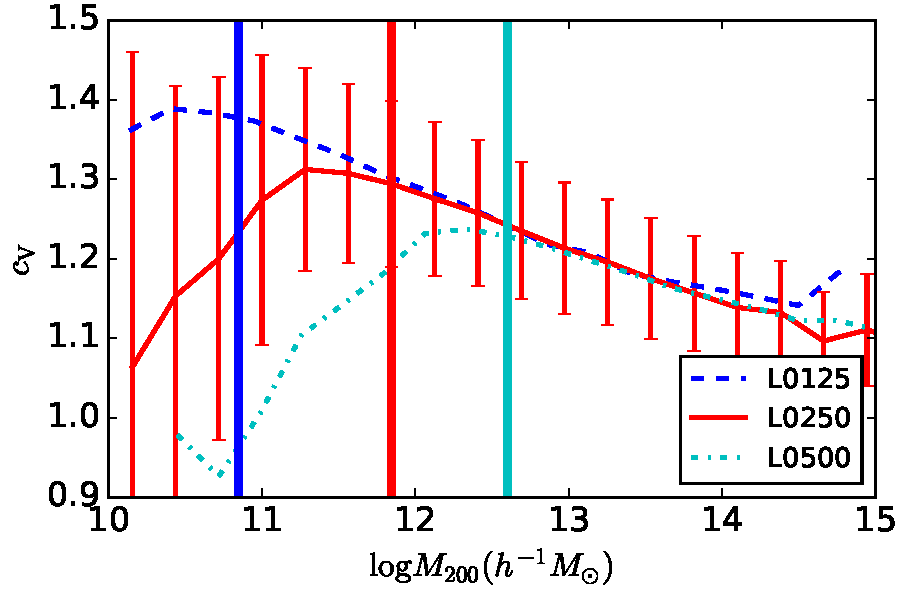
\includegraphics[width=.5\textwidth]{masscut_cV_d200.pdf}
\caption{The relationship between the velocity ratio concentration and halo mass for each of our simulations with $\Delta =200$. 
In order of increasing simulation volume, the blue line corresponds to the concentration-mass relation from simulation 
\simA, the red line corresponds to \simB, and the cyan line corresponds to \simC. The red error bars show the 68\% spread in
parameter values within that mass bin for \simB. These errors are comparable to those of the other simulations
within the region of interest.
Each simulation is subject to resolution limitations at different halo masses. We show with arrows
the minimum $M_{200}$ mass thresholds that we adopt in our analyses using the same color code as 
the concentration-mass relations, going from \simA \ to \simC \ from left to right. Note the deviation from a monotonic trend as a result of resolution effects.
}
\label{fig:cvrelation}
\end{figure}
%--------------------------------------------------------------------------------

%-------------------------------------------- Figure comparing Cnfw and Cv on a halo-by-halo basis
\begin{figure}
\centering
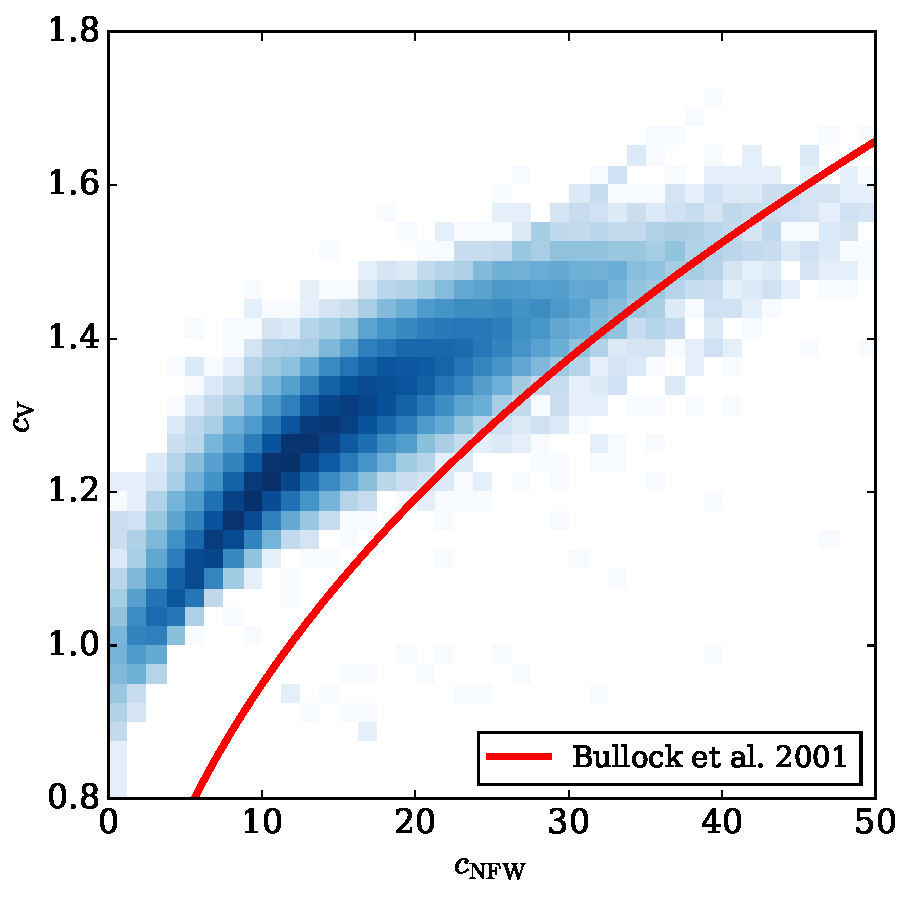
\includegraphics[width=.5\textwidth]{cvvscnfw_relation.pdf}
\caption{
The relationship between the two different measures of concentration, 
using halos in \simB. The color scale, shown at the right, encodes the number of halos 
within a single two-dimensional bin in the $c_{\mathrm{NFW}}$-$c_{\mathrm{V}}$ space. 
The red (blue) regions on the plot show where the most (fewest) halos exist with those values of the two
concentration parameters. The white regions indicate where no halos hold these values. The scatter on this relationship ranges from 5\% for intermediate concentration values, to a high of 13\% at high masses.
}
\label{fig:concentrations}
\end{figure}
%--------------------------------------------------------------------------------------------------------------------------------


%---------------------------------------
\subsection{Halo Shape}

In addition to halo concentrations, we examine halo clustering as a function of a variety of other 
halo properties. We study halo clustering as a function of halo shape, $s$, 
quantified by the ratio of the halo minor, $c$ and major axis, $a$, lengths, 
%
\beq
s = \frac{c}{a}.
\eeq
%
The halo shapes we used were measured with {\tt ROCKSTAR} by calculating the mass distribution tensor,
\beq
M_{ij}=\frac{1}{N}\sum\limits_{N}x_i x_j,
\eeq
for
all particles within the halo radius, excluding identified substructure. The sorted eigenvalues of the matrix represent
the squares of the principal ellipsoid axes, where a \textgreater b \textgreater c. \asv{Not sure if I should include the equation for the mass distribution tensor.} \arz{Yes, put in the equation. Also, I don't think your statement about rockstar excluding substructure is accurate. Is it? Please check on this.}\asv{I am entirely sure that for the shape parameters substructure is excluded by {\tt ROCKSTAR}.} The mean relations for halo shapes as a function of halo mass for $\Delta=200$ are shown in Figure~\ref{fig:srelation} along with the mass 
thresholds used to ensure that our results are not compromised by 
resolution.


%------------------------------------------ Figure for s(M)
\begin{figure}
\centering
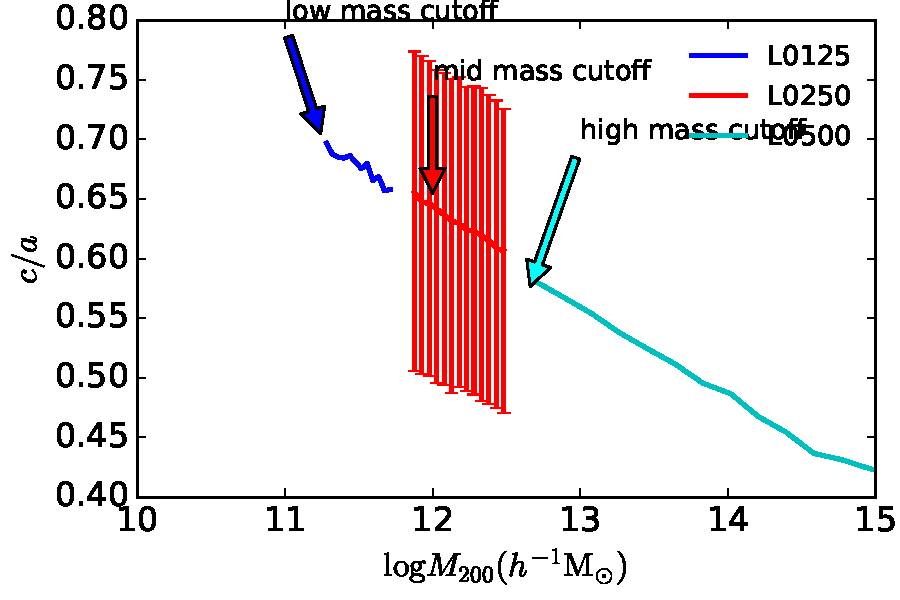
\includegraphics[width=.5\textwidth]{masscut_shape_d200.pdf}
\caption{
The relationship between the halo shape and halo mass for each of our simulations with $\Delta =200$. 
In order of increasing simulation volume, the blue line corresponds to the shape-mass relation from simulation 
\simA, the red line corresponds to \simB, and the cyan line corresponds to \simC. The red error bars show the 68\% spread in
parameter values within that mass bin for \simB. These errors are comparable to those of the other simulations
within the region of interest.
Each simulation is subject to resolution limitations at different halo masses. We show with arrows 
the minimum $M_{200}$ mass thresholds that we adopt in our analyses using the same color code as 
the shape-mass relations, going from \simA \ to \simC \ from left to right. The mass cutoffs chosen for this mark
are at higher masses in order to account for the additional number of particles needed to properly measure the
halo shape. Note the deviation from a monotonic trend as a result of resolution effects.
}
\label{fig:srelation}
\end{figure}
%--------------------------------------------------------------------------------

%-----------------------------
\subsection{Halo Spin}

We study halo clustering as a function of halo angular momentum quantified 
by the spin parameter, $\lambda$, as introduced by \citep{peebles69},
\beq
\lambda = \frac{J \sqrt{\lvert E\rvert}}{G M_{\Delta}^{2.5}}
\eeq
where $J$ is the halo angular momentum, $E$ is the total energy of the 
halo, and $M_{\Delta}$ is the mass at the halo radius, $r_{\Delta}$. We measure this quantity using {\tt ROCKSTAR} which calculates the angular momentum, total energy, and total mass within $\Delta$ using bound particles out to the corresponding halo radius.
The mean relations for halo spin as a function of halo mass for $\Delta=200$ are shown in Figure~\ref{fig:spinrelation} along with the mass thresholds enforced to ensure that our results are not compromised by resolution. These thresholds are summarized in Table~\ref{table:thresholds}, where we also show the threshold masses at various values of the overdensity parameter, $\Delta$.

%------------------------------------------ Figure for lambda(M)
\begin{figure}
\centering
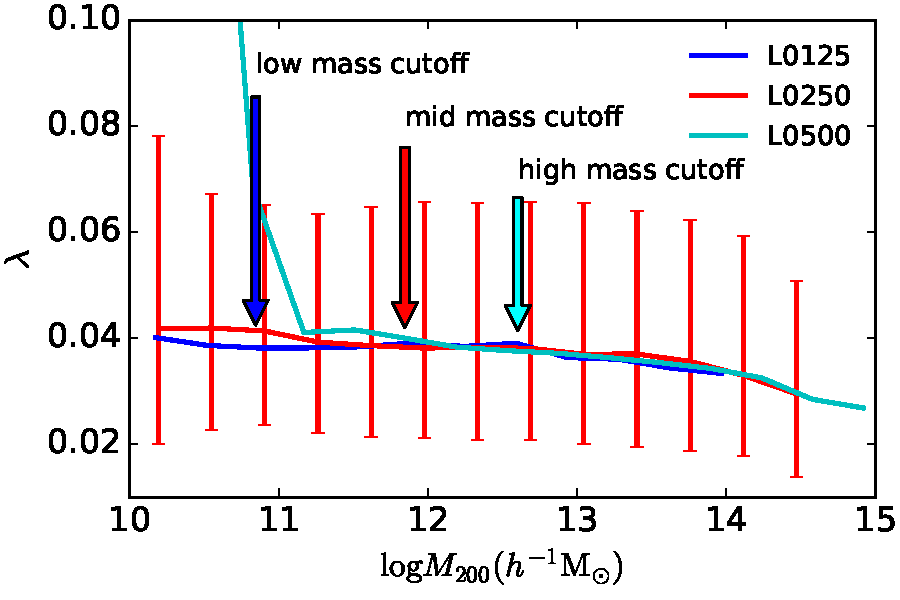
\includegraphics[width=.5\textwidth]{masscut_spin_d200.pdf}
\caption{
The relationship between the halo spin and halo mass for each of our simulations with $\Delta =200$. 
In order of increasing simulation volume, the blue line corresponds to the spin-mass relation from simulation 
\simA, the red line corresponds to \simB, and the cyan line corresponds to \simC. The red error bars show the 68\% spread in
parameter values within that mass bin for \simB. These errors are comparable to those of the other simulations
within the region of interest.
Each simulation is subject to resolution limitations at different halo masses. We show with arrows 
the minimum $M_{200}$ mass thresholds that we adopt in our analyses using the same color code as 
the spin-mass relations, going from \simA \ to \simC \ from left to right. Note the deviations from the near linear trend at low mass due to resolution effects.}
\label{fig:spinrelation}
\end{figure}
%--------------------------------------------------------------------------------

%---------------------------------
\subsection{Halo Samples}

In practice, the mean relations between the various halo properties and the mass 
thresholds for our analyses must be determined separately for each combination of simulation, 
halo property (e.g., $c_{\mathrm{NFW}}$ or $s$), and halo definition (i.e., value of $\Delta$ in the case of the present study). 
For each analysis, we set mass thresholds in order to avoid the regime in which 
halo parameters are not well measured due to resolution limits of the simulations; 
we draw attention to the downturn in Figure~\ref{fig:cnfwrelation} as an example of this, 
as the deviation from the underlying monotonic trend shifts with the change in 
simulation from lower to higher resolution, suggesting that this is the result of resolution alone. 


For ease of comparison between halo definitions, we choose to use a single mass threshold for each
simulation and value of $\Delta$ whenever possible, rather than on a parameter-by-parameter basis. 
The one exception to this method is the mass thresholds chosen
for the halo shape parameter. This parameter requires a larger number of particles to be
well measured; we direct attention to the downturn in Figure~\ref{fig:srelation}, which occurs at
a significantly higher mass than demonstrated with other halo properties (see Figure~\ref{fig:cnfwrelation}
for comparison). We analyze the shape parameter with separate, larger minimum mass thresholds to account for 
the requirement for a larger number of particles. This allows us
to have better signal-to-noise in the remaining parameters, while avoiding drawing potentially
erroneous conclusions when analyzing the halo shape parameter.
We summarize the mass thresholds we have used for a 
subset of $\Delta$ values in Table~\ref{table:thresholds}. 
At most values of $\Delta$, the minimum mass thresholds are 
driven by the requirement that the halo properties do 
not suffer significantly from finite resolution effects. We alert the reader to the fact 
that the mass of an individual halo will vary as $\Delta$ varies. This effect can be seen in Figure~\ref{fig:massmatch}, which demonstrates that while a decreased value of $\Delta$ leads to larger masses on average, there is a scatter due to changes in halo identification. Roughly speaking, 
the threshold masses in Table~\ref{table:thresholds} vary in such a way that the 
same physical objects are selected at each halo definition.

\begin{figure}
\centering
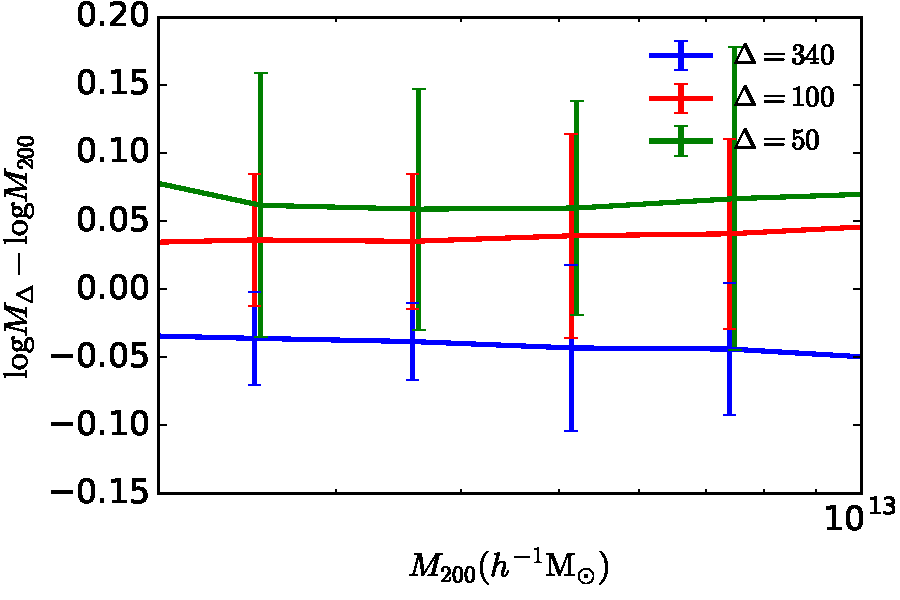
\includegraphics[width=.5\textwidth]{massdeltacompare.pdf}
\caption{
The logarithmic difference between host halo mass for a given definition of $\Delta$ and the equivalent halo for a definition of $\Delta=200$ in logarithmic space. The blue (red, green) lines look at the ratio with respect to the values of $\Delta=340$ ($100, 50$). Error bars show one standard deviation of the distribution in that mass bin. Note that while the expectation is that the halo mass will be larger for lower values of $\Delta$, there are some differences due to differences in halo identification. 
\arz{Several comments. First, plot $\log(M_{\Delta}/M_{200})$ because 
$M_{200}$ is the quantity people will be familiar with. Second, you should compute these ratios from the ``matched'' catalogs! That way there is no issue of having the ratio affected by including or excluding certain halos. Third, you have to specify what the lines and errorbars are? Are they mean and scatter? Lastly, I think it is best if the x-axis is logarithmic. Most of your data is piled up against the y-axis here because that is where most of yourh halos are! A logarithmic x-axis running from $\sim 10^{11}$ to $\sim 10^{14}$ seems most sensible to me.}
}
\label{fig:massmatch}
\end{figure}





%%%%%%%%%%%%%%%%%%%%%%%%%%%%%%%%%%%%%%%%%%%%%%%%%%%%%%%%%%%%%%%%%%%%%%%%%%%%
\begin{table*}
\caption{
Minimum mass thresholds for each of our analyses. 
In the columns below each value of $\Delta$, we show the minimum 
host halo masses considered in units of $h^{-1}\mathrm{M}_{\odot}$.
Those rows without a label of ``-shape" refer to the mass cut chosen for 
all analyses other than halo shape. Those rows with a label of ``-shape" refer to 
the mass cut chosen for the shape parameter analyses. The latter require higher mass thresholds.}
\vspace*{8pt}
\begin{tabular}{ c c c c c c c }
\hline
\hline
Cutoff Name &  $\Delta=340$ & $\Delta=200$ & $\Delta=100$ & $\Delta=75$ & $\Delta=50$ & $\Delta=10$ \\
\hline
\vspace*{2pt}
{low mass} & $6 \times 10^{10}$ & $7 \times 10^{10}$ & $8 \times 10^{10}$ & $9 \times 10^{10}$ & $1 \times 10^{11}$ & $2 \times 10^{11}$  \\ \vspace*{4pt}
{low mass-shape} & $2 \times 10^{11}$ & $2 \times 10^{11}$ & $2 \times 10^{11}$ & $2 \times 10^{11}$ & $2 \times 10^{11}$ & $2 \times 10^{11}$ \\
{mid mass} & $6 \times 10^{11}$ & $7 \times 10^{11}$ & $8 \times 10^{11}$ & $9 \times 10^{11}$ & $2 \times 10^{12}$ & {N/A} \\ \vspace*{4pt}
{mid mass-shape} & $2 \times 10^{12}$ & $2 \times 10^{12}$ & $2 \times 10^{12}$ & $2 \times 10^{12}$ & $2 \times 10^{12}$ & {N/A} \\
{high mass} & $3 \times 10^{12}$ & $4 \times 10^{12}$ & $5 \times 10^{12}$ & $6 \times 10^{12}$ & $7 \times 10^{12}$ & {N/A} \\ \vspace*{2pt}
{high mass-shape} & $1 \times 10^{13}$ & $1 \times 10^{13}$ & $1 \times 10^{13}$ & $1 \times 10^{13}$ & $1 \times 10^{13}$ & {N/A} \\
\hline
\hline \\
\end{tabular}
\label{table:thresholds}
\end{table*}
%%%%%%%%%%%%%%%%%%%%%%%%%%%%%%%%%%%%%%%%%%%%%%%%%%%%%%%%%%%%%%%%%%%%%%



%-----------------------
\section[]{Halo Clustering as a function of Auxiliary Halo Properties}
\label{section:methodology}
%-----------------------

%----------------------------------------------------------
\subsection{Auxiliary Halo Properties and Their Mass Dependence}
\label{subsection:properties}

We are interested in studying the clustering behavior of halos as a function of 
properties other than mass. As mass is the dominant halo property determining halo
clustering strength and environment, we refer to the other properties that we study as 
``auxiliary halo properties" (those properties other than mass, such as concentration 
$c_{\rm NFW}$ or shape $s$). As has been demonstrated extensively in the literature, 
the auxiliary properties that we consider are themselves 
a function of mass \citep{bullock_etal02,allgood_etal06, duffy_etal08, despali_etal16}. 
This mass dependence, if not accounted for, induces clustering that depends upon these auxiliary properties in the absence of assembly bias. 
Most contemporary cosmological $N$-body simulations, and specifically the suite of simulations 
that we study in this work, do not have a sufficiently large number of halos to make isolating halos 
of fixed mass, and then further splitting these halos by an auxiliary property, a statistically 
powerful method with which to study the dependence of clustering on auxiliary properties. 
Therefore, it is necessary to remove and/or mitigate the mass dependence of the auxiliary 
properties that we study. 

We mitigate the mass dependence of the auxiliary properties as follows. First, 
we take all host halos more massive than our minimum mass thresholds and sort them by 
their halo masses, $M_{\Delta}$. We place these halos into twenty logarithmically-spaced bins 
of halo mass, ensuring that no bin has fewer than 10 halos, with the exception of the most massive bin. The objects in this final bin are rare and exceptional enough that they have little statistical value and do not influence our results considerably. 
We then calculate the rank of each auxiliary property within the bin of halo mass, from 1 to N, where N is the number of halos assigned to a given bin. If multiple halos share auxiliary property values (e.g. rank 2 and 3 have the same halo shape), then the average value of the rank is assigned to each halo (e.g. 2.5 to each). We normalize the rank distribution to be between 0 and 1 by dividing out the number of halos in the bin. This removes the strong mass trend in each of these properties. We use these normalized ranks of halo auxiliary properties to study halo clustering strength in the remainder of this work. We have experimented with different bin sizes. We find that our qualitative results are not sensitive to the number of bins we use. Furthermore, the choice of equally populated bins versus evenly spaced bins makes no significant difference to our results.

In addition to the properties of the host halos described in the previous section, we also study the strength of halo clustering as a function of subhalo number. Host halo size and the number of satellite halos (above some threshold in a proxy of satellite halo size) 
are also strongly correlated. Roughly speaking, the number of satellite halos above a fixed size threshold grows in approximate proportion to host halo mass \cite{zentner_etal05}. \arz{Cite Kravtsov et al. 2003 here.}

To account for the correlation between halo mass and abundance of subhalos, we follow the prescription of \citet{wechsler_etal06}. We first select all subhalos from the sample
that meet the criterion that the ratio $V_{\mathrm{max,sub}}/V_{\mathrm{max,host}} \ge 0.3$, where
$V_{\mathrm{max,sub}}$ and $V_{\mathrm{max,host}}$ are the maximum circular velocities of the subhalos and host halos respectively.
This choice of scaling exploits the fact that the subhalo velocity function is a very nearly self-similar function \citep{zentner_etal05}
so that the scaling eliminates the gross mass dependence of satellite number. \asv{need to add in additional citations here.} 
In addition, this choice of threshold will mean that for subhalos above the resolution threshold of the simulation, there shall be of order a few satellite halos per host on average. We then choose
a threshold for the host maximum circular velocity such that all subhalos are well-resolved in the simulation volumes: $135, 235$, and $400 \mathrm{km \ s^{-1}}$ for \simA, \simB, and \simC~ respectively. Subhalo maximum circular velocities were used as a proxy for subhalo size rather than subhalo masses because subhalo maximum circular velocities can be more robustly measured from simulation data, making comparison to other work easier. Once these cuts have been applied, we again divide the halos that meet these cutoffs into bins in logarithmic halo mass and follow the same procedure as with the other auxiliary halo properties. \arz{Now that you use ranks, this means you are "doubly" removing the mass dependence. This is OK. It just may not be necessary now that you have moved to using ranks.}\asv{Probably not necessary, though it does serve as an informed cut on minimum subhalo mass, so I will leave it in.}

%---------------------------------------------------------------
\subsection{Clustering Statistics}
\label{subsection:clusteringstatistics}
%---------------------------------------------------------------


We assess the influence of assembly bias specifically on two-point statistics of host halos. In order to do so, we 
study both the standard two-point correlation functions of halos selected by properties other than mass 
(e.g., the auxiliary properties concentration, shape, and spin) as well as halo mark correlation functions
(MCFs). MCFs quantify the manner in which a halo property (the ``mark") correlates among halo pairs as a function
of the distance between the pairs. MCFs have the advantage that they effectively stack signal from all values of 
the halo auxiliary property, or mark, in contrast to selecting subsets of halos based on the auxiliary property. 
MCFs also stack signal from all environments and do not require any specific definition of halo environment in 
order to detect ``environmental" trends that are usually referred to as assembly bias in the literature. 
Absent halo assembly bias, the halo marks are uncorrelated among pairs. 
MCFs have been used in many previous papers to quantify environmental dependence of halo 
properties other than mass \citep{sheth_tormen04,sheth05, harker_etal06,wechsler_etal06,mao_etal15}. 
Although it does not necessarily have to be the case, we find that using correlation functions of halo sub-samples 
and using MCFs lead to the same broad conclusions. 


For a specific halo property, or mark $m$, we use the MCF normalization of \citet{wechsler_etal06}, namely 
%
\beq
\mathcal{M}_m(r) \equiv \frac{\langle m_1 m_2 \rangle_p (r) - \langle m \rangle^2}{\mathcal{V}(m)},
\eeq
%
where $m_{\mathrm{i}}$ is the value of the mark for halo $\mathrm{i}$, $\langle m \rangle$ is the mean of the
mark, and $\mathcal{V}(m)$ the variance of the mark. The notation is intended to indicate that the average is
taken over all pairs of halos separated by a distance $r$. In the absence of any correlation between a halo
property among neighbors a separation $r$ away, $\mathcal{M}_m(r) = 0$. Deviations of the MCF from
zero indicate such correlations exist and the magnitude of $\mathcal{M}_m(r)$ gives the excess of the mark among
pairs compared to the one-point mean of the mark $\langle m\rangle$ in units of the one-point variance. The marks that we use are the 
normalized ranks of halo auxiliary properties described in Section~\ref{subsection:properties}. Therefore, these marks are distributed according 
to a uniform distribution from 0 to 1, so that $\langle m \rangle^2 = 0.25$ and that $\mathcal{V}(m) = 1/12$. 


In each case, it is necessary to assess statistical fluctuations in the statistics that we measure in these simulations in
order to determine the significance of the signals. For two-point correlation functions, we determine the
covariance of the measurement through jackknife resampling of the eight octants of the simulation cube. 

\arz{After the discussions that we had, is this still what you are doing?}\asv{No it is not! I missed changing it!}
We assess the significance of the MCFs by taking advantage of the inherent uniform distribution. For each halo we assign a random mark drawn from a uniform distribution. We repeat this process 200 separate times and calculate the MCF for each set of random marks. From this distribution of MCF values, we take the 2\% and 98\% percentile values in order to create a range which should correspond well with a 2 $\sigma$ interval; we propose that a signal within this range could not be positively identified as assembly bias. We note that since we investigate the product of two uniformly distributed variables, a negative value of the MCF has two different interpretations. One interpretation is that halos with high (low) values of the mark experience enhanced (diminished) clustering. The other possible interpretation is an enhanced clustering of high value marks with low value marks. While we cannot distinguish between these two possibilities, it does not impact our ability to make statements about a potential non-detection of assembly bias, as our randomization implicitly accounts for the impact of a uniform product distribution.


%----------------------------
\section[]{Results}
\label{section:results}
%----------------------------


%-----------------------------------------------
\subsection{Correlation Functions}
\label{sub:cfresults}


We begin by studying the correlation functions of halos in our mass threshold samples, sub-selected by auxiliary
properties. Figure~\ref{fig:cc_cfcompare} exhibits the difference between the clustering strength of halos in the
$20^{\mathrm{th}}$ percentile highest NFW concentrations and the halos with the halos that have the
$20^{\mathrm{th}}$ percentile lowest NFW concentrations as a function of the overdensity parameter, $\Delta$, used to
define the halos. In order to make the differences more apparent, the two-point functions in 
Fig.~\ref{fig:cc_cfcompare} have been normalized by the clustering strength of the entire halo sample. 


If the clustering strength of halos were independent of halo concentration, we 
would expect the lines in Fig.~\ref{fig:cc_cfcompare} to cluster around zero (scattered about zero by finite sample size). 
The evident deviations demonstrate that halos of different NFW concentrations exhibit appreciably 
different clustering, a fact that is already well known and has been studied by a number of authors. 
Furthermore, it is clear that the strength and sign of assembly bias due to NFW concentration is 
strongly mass dependent for any fixed halo definition, a result that also agrees with the significant 
previous literature on halo assembly bias using conventional halo definitions 
\citep{wechsler_etal02, gao_etal05, zentner07, wechsler_etal06, harker_etal06, croton_etal07, dalal_etal08, mao_etal15, sunayama_etal16}.
At relatively low mass (the low-mass panel, $M_{200} > 7 \times 10^{10} \hMsun$), 
high-concentration halos are considerably more strongly clustered than low-concentration halos using the more 
conventional $\Delta = 200$ definition for halos. At somewhat higher halo masses 
(e.g., the mid-mass panel, $M_{200} > 7 \times 10^{11} \hMsun$), this difference is markedly reduced. 
Finally, for the highest-mass halos that we have the capability of studying (the high-mass panel, 
$M_{200} > 4 \times 10^{12} \hMsun$), the effect is weaker and also of opposite sign; 
low-concentration halos are more strongly clustered than high-concentration halos.

Focus, for example, on the middle panel of Fig.~\ref{fig:cc_cfcompare}. In this panel, 
corresponding to the mid-mass threshold, the difference in large-scale clustering between 
high- and low-concentration halos is dramatically reduced for a halo definition with 
$\Delta \approx 60$ as compared to a more traditional halo definition, such as $\Delta=200$. 
However, further decreasing $\Delta$ leads to concentration-dependent clustering of opposite sign. 
Both the strength and the sense of halo assembly bias depend upon halo definition! This is a 
point that may seem somewhat obvious in retrospect, but does not seem to be addressed 
explicitly anywhere in the literature despite its importance.


Comparing the differing clustering strengths across the three panels of Fig.~\ref{fig:cc_cfcompare}, 
it is clear that any specific conclusions about concentration-dependent halo clustering 
vary with halo mass. For low-mass halos (the top panel), 
very low values of $\Delta$ (and correspondingly large definitions of halo radii, 
as $R_{\Delta}$ very roughly in proportion to $\Delta^{-1/3}$) are necessary in order 
to mitigate the concentration dependence of halo clustering. Conversely, for higher-mass 
halos (the bottom panel), conventional values of $\Delta \sim 200-340$ yield little 
concentration-dependent clustering. In this case, decreasing $\Delta$ (increasing $R_{\Delta}$) 
results in significantly {\em increased} concentration dependent halo clustering. The reasons for 
these changes are of interest and we return to the interpretation of these results below.


Notice that in all panels of Fig.~\ref{fig:cc_cfcompare}, the effect of concentration-dependent clustering is
mildly scale-dependent. Moreover, this scale dependence is evident for all values of $\Delta$. Simply
defining halos with a different value of $\Delta$ does not suffice to eliminate concentration-dependent
clustering on all scales. In this discussion and throughout, we focus primarily on the large scale clustering,
which we take to mean clustering on scales significantly larger than the radii, $R_{\Delta}$ of the halos in our
samples.


%---------------------------------------------------------------------------------------------------------------------------------------
\begin{figure}
	\centering
	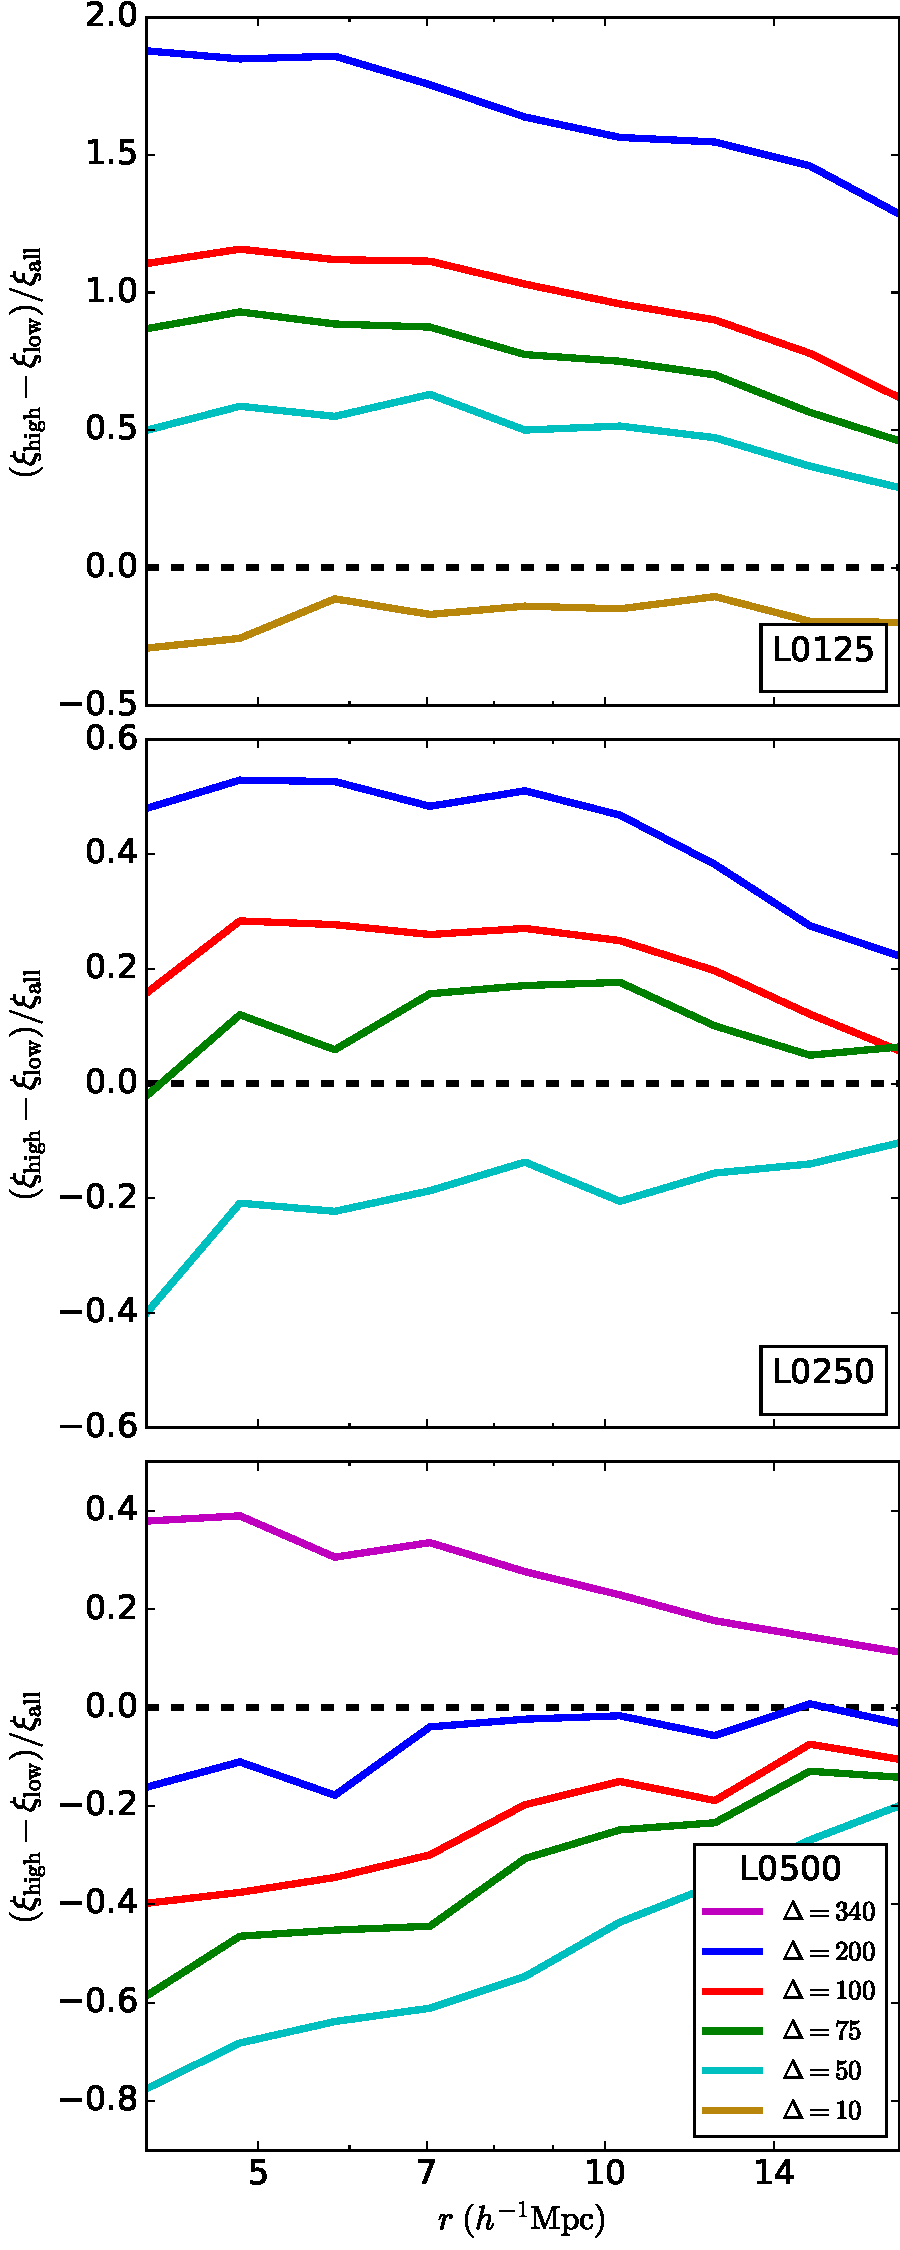
\includegraphics[width=.4\textwidth]{all_cfcompare_cnfw.pdf}
	\caption{
In each panel, the solid lines plot the difference between the correlation function for the top
20\% and the bottom 20\% of halos by NFW concentration, normalized by the
correlation function of the entire sample. In each plot the lines correspond to different values of $\Delta$, with dark blue (light blue) corresponding to $\Delta = 340$ ($\Delta = 50$). The 
 line corresponds to the overdensity chosen for matching as possibly removing assembly bias on most scales in the case of halo concentration.
The top (middle/bottom) panel shows the results for the \simA \ (\simB /\simC) data 
set utilizing the low mass (mid mass/high mass) cutoffs. Error bars correspond to the two $\sigma$ error on the measurement.
}
\label{fig:cc_cfcompare}
\end{figure}
%----------------------------------------------------------------------------------------------------------------------------------------------


It should be noted that this method is robust to the choice of samples. For instance, 
changing from examining the $20^{\mathrm{th}}$ percentile of concentrations to another 
value (e.g., $10^{\mathrm{th}}$ or $50^{\mathrm{th}}$ percentile) 
does not change the conclusions drawn from Fig.~\ref{fig:cc_cfcompare} significantly. In the 
case of halo concentration, adopting $c_{\mathrm{V}}$ rather than $c_{\mathrm{NFW}}$ 
also does not alter our conclusions. Therefore, we do not show these additional results 
in the interest of brevity.

Furthermore, we note that quite generally, for each of the halo properties we have studied, 
the conclusions drawn from examining correlation functions are the same as those drawn from 
studying MCFs. Consequently, we now move on to a more comprehensive 
discussion of the strength of auxiliary property-dependent halo clustering using MCFs. 


%-----------------------------------------------------------------
\subsection{Mark Correlation Functions}
\label{sub:mcfresults}

\begin{figure}
	\centering
	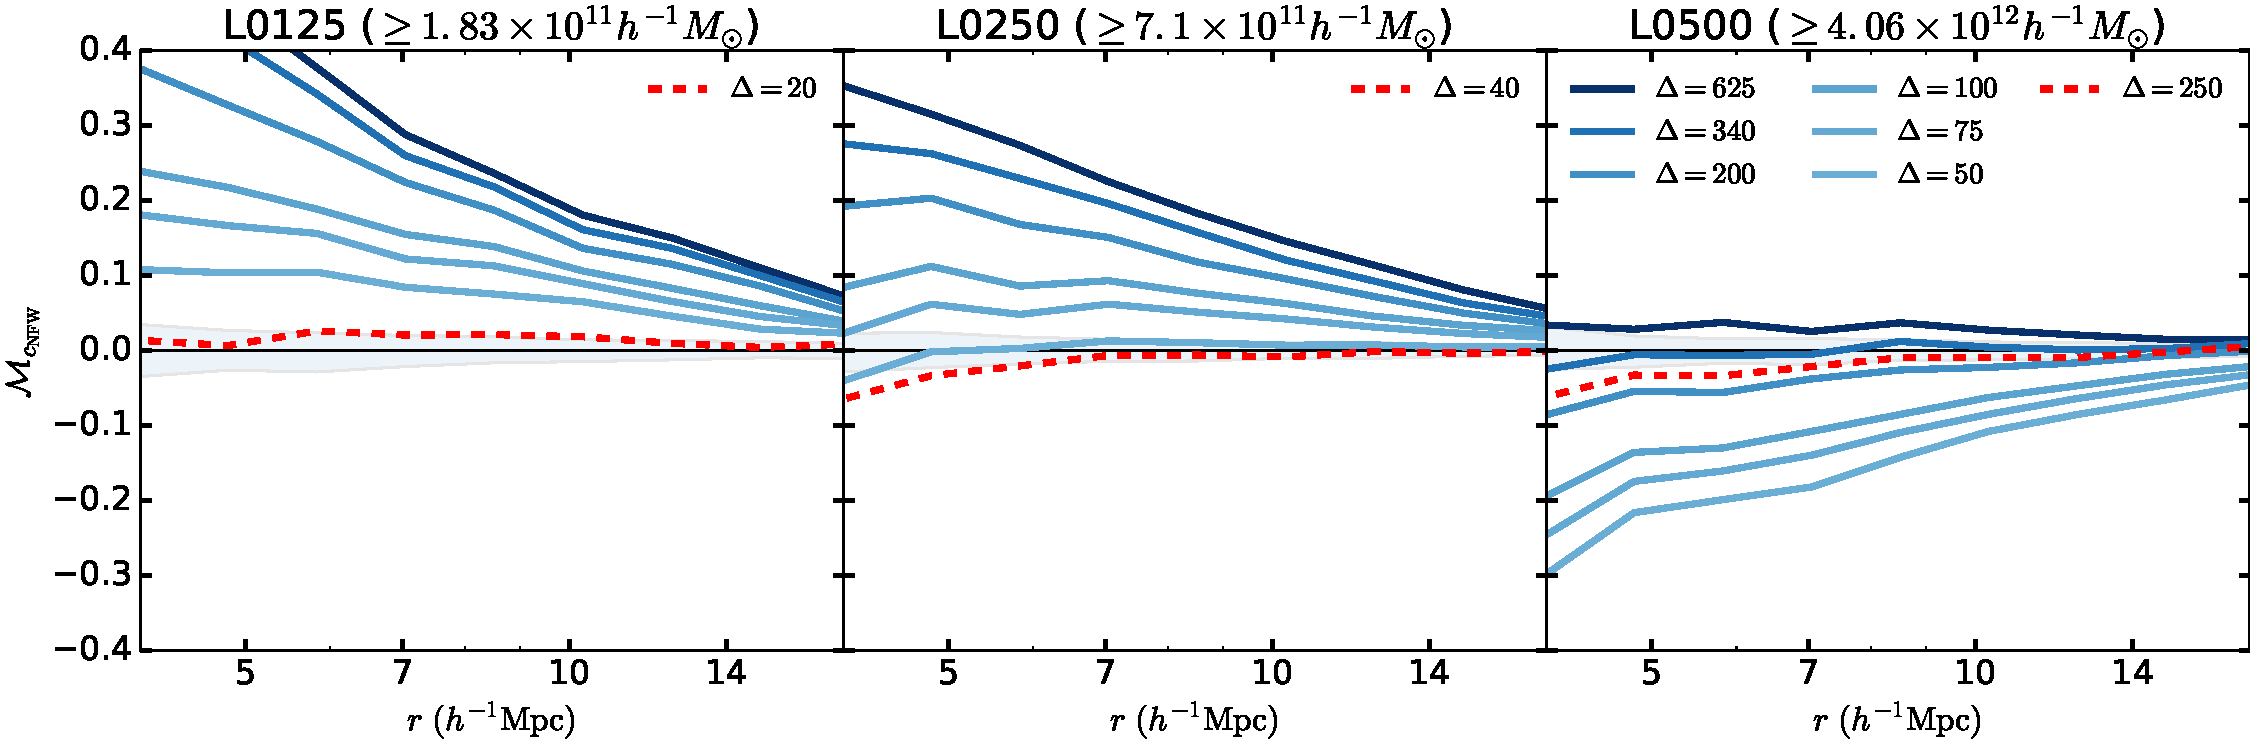
\includegraphics[width=.4\textwidth]{all_mcf_cNFW.pdf}
	\caption{
The marked correlation function for the concentration defined according to the NFW profile. The solid lines plot the marked correlation function using normalized ranks of NFW concentration as the mark. In each plot the lines correspond to different values of $\Delta$, with dark blue (light blue) corresponding to $\Delta = 340$ ($\Delta = 50$). The red dashed line corresponds to the overdensity chosen for matching as possibly removing assembly bias on most scales in the case of halo concentration. The top (middle/bottom) panel shows the results for the\simA \ (\simB /\simC) data set utilizing the low mass (mid mass/high mass) cutoffs. The shaded bands represent 2-sigma confidence regions generated by randomization of the marks.
}
	\label{fig:cc_mcf_cnfw}
\end{figure}


%------------------------
\subsubsection{Halo Concentration}

The NFW concentration, $c_{\mathrm{NFW}}$, MCF is shown in Figure~\ref{fig:cc_mcf_cnfw}. 
The shaded bands in the figure delineate the statistical fluctuations in MCFs induced by 
finite sampling as discussed in Section~\ref{subsection:clusteringstatistics}. 
Qualitatively, Fig.~\ref{fig:cc_mcf_cnfw} exhibits the same features that are evident in 
Fig.~\ref{fig:cc_cfcompare}: more concentrated halos are significantly more clustered in 
the low-mass cut L0125 halo sample; concentration-dependent halo clustering weakens and 
reverses sense as halo mass increases (at fixed $\Delta$), 
consistent with work on assembly bias \citep{wechsler_etal06,sunayama_etal16}; for the 
mid-mass cut L0250 sample with $\Delta=60$, the large-scale concentration dependence of halo clustering has been reduced so as to 
be consistent with zero within the statistical limitations of the simulation. 

Figure~\ref{fig:cc_mcf_cV} is a similar plot for the MCF of the velocity-ratio concentration, $c_{\mathrm{V}}$. 
This figure exhibits qualitatively very similar features to Fig.~\ref{fig:cc_mcf_cnfw}, a 
fact that is not surprising given that we already know that $c_{\mathrm{NFW}}$ and $c_{\mathrm{V}}$ 
quantify largely redundant information about their halos.

%---------------------------------------------------
\begin{figure}
	\centering
	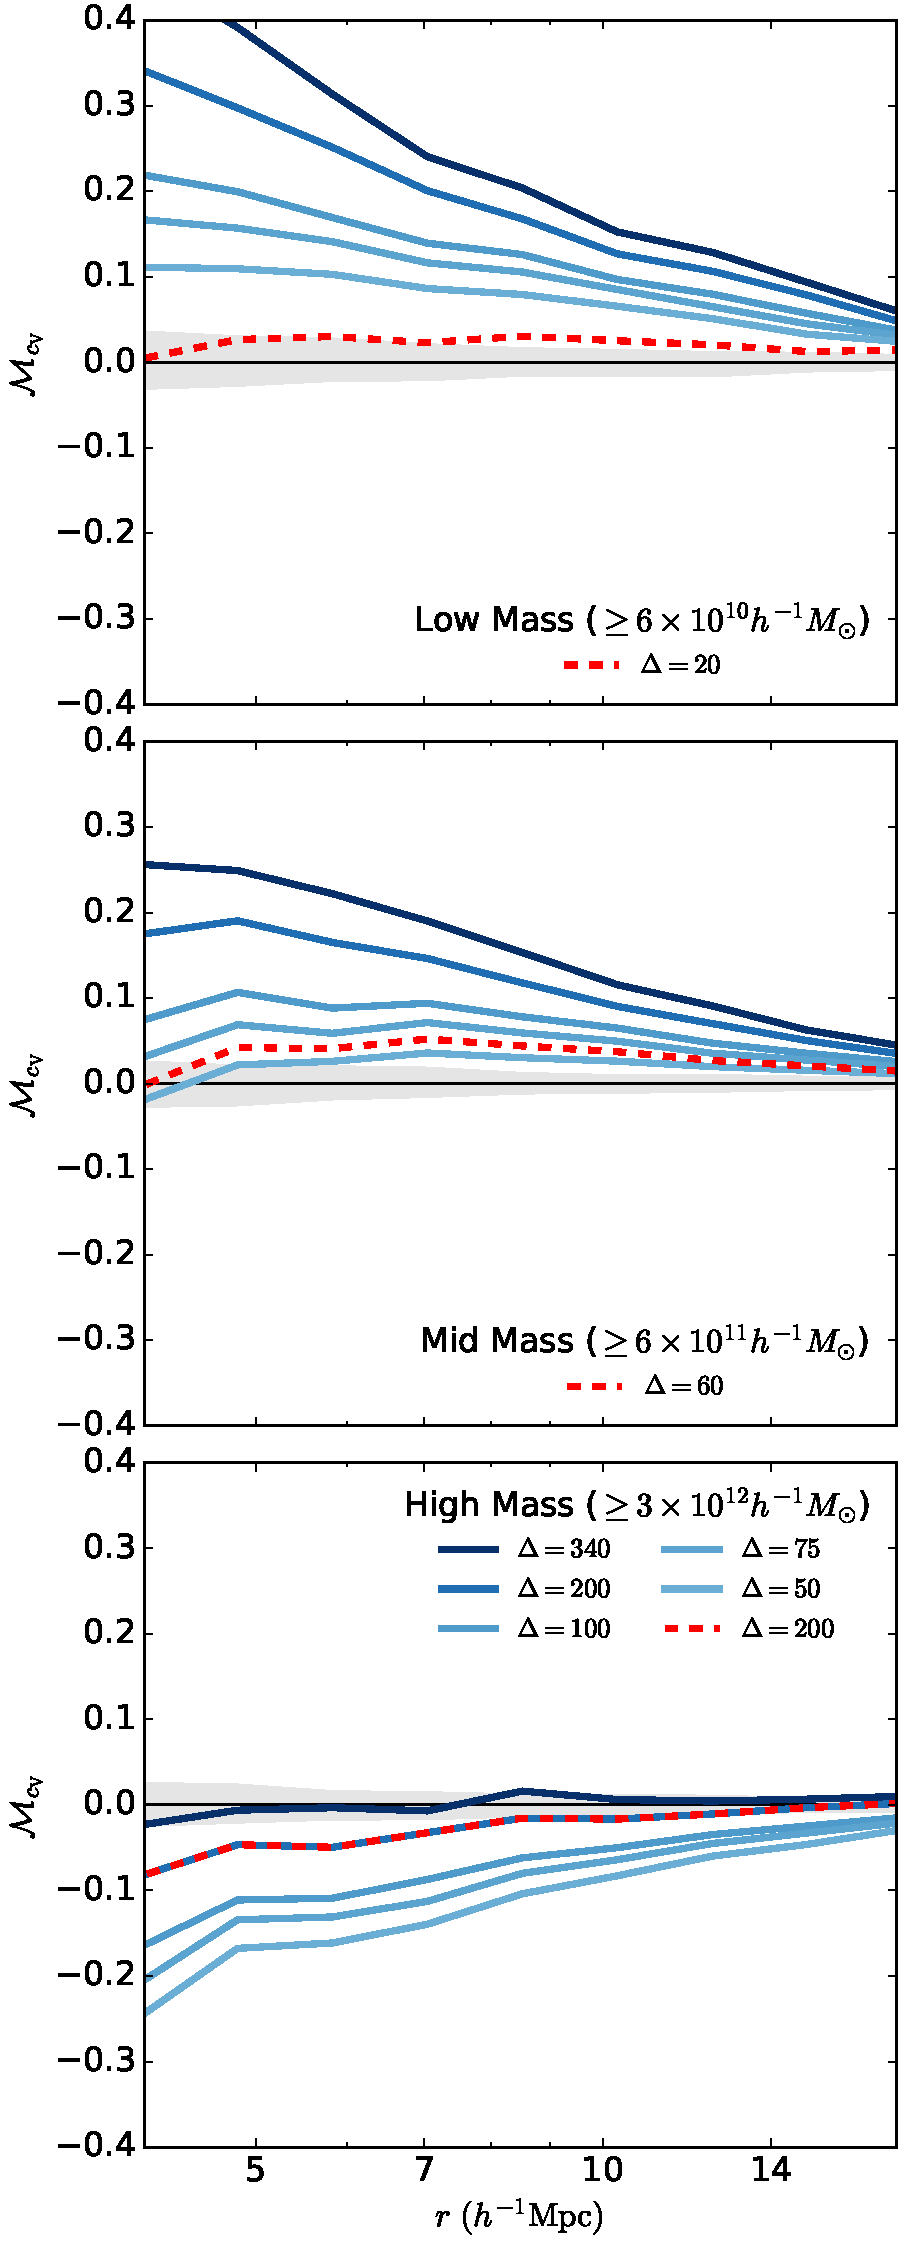
\includegraphics[width=.4\textwidth]{all_mcf_cV.pdf}
	\caption{	
The marked correlation function for the concentration defined according to the ratio of maximum circular velocities. The solid lines plot the marked correlation function using velocity ratio concentration as the mark. In each plot the lines correspond to different values of $\Delta$, with dark blue (light blue) corresponding to $\Delta = 340$ ($\Delta = 50$). The red dashed line corresponds to the overdensity chosen for matching as possibly removing assembly bias on most scales in the case of halo concentration. The top (middle/bottom) panel shows the results for the
\simA \ (\simB /\simC) data set utilizing the low mass (mid mass/high mass) cutoffs. The shaded bands represent 2-sigma confidence regions generated by randomization of the marks. 
\arz{Still have to play with the cosmetics of this plot a little. Too much data is cut our of the top panel. Maybe extend the vertical axis to about 0.4 or so? Then it would have the same dynamic range as the NFW concentration plot, which would be nice!}\asv{Changes made!}
}
	\label{fig:cc_mcf_cV}
\end{figure}
%---------------------------------------------------


%----------------------
\subsubsection{Halo Shape}

%--------------------------------------------------- Shape MCFs
\begin{figure}
	\centering
	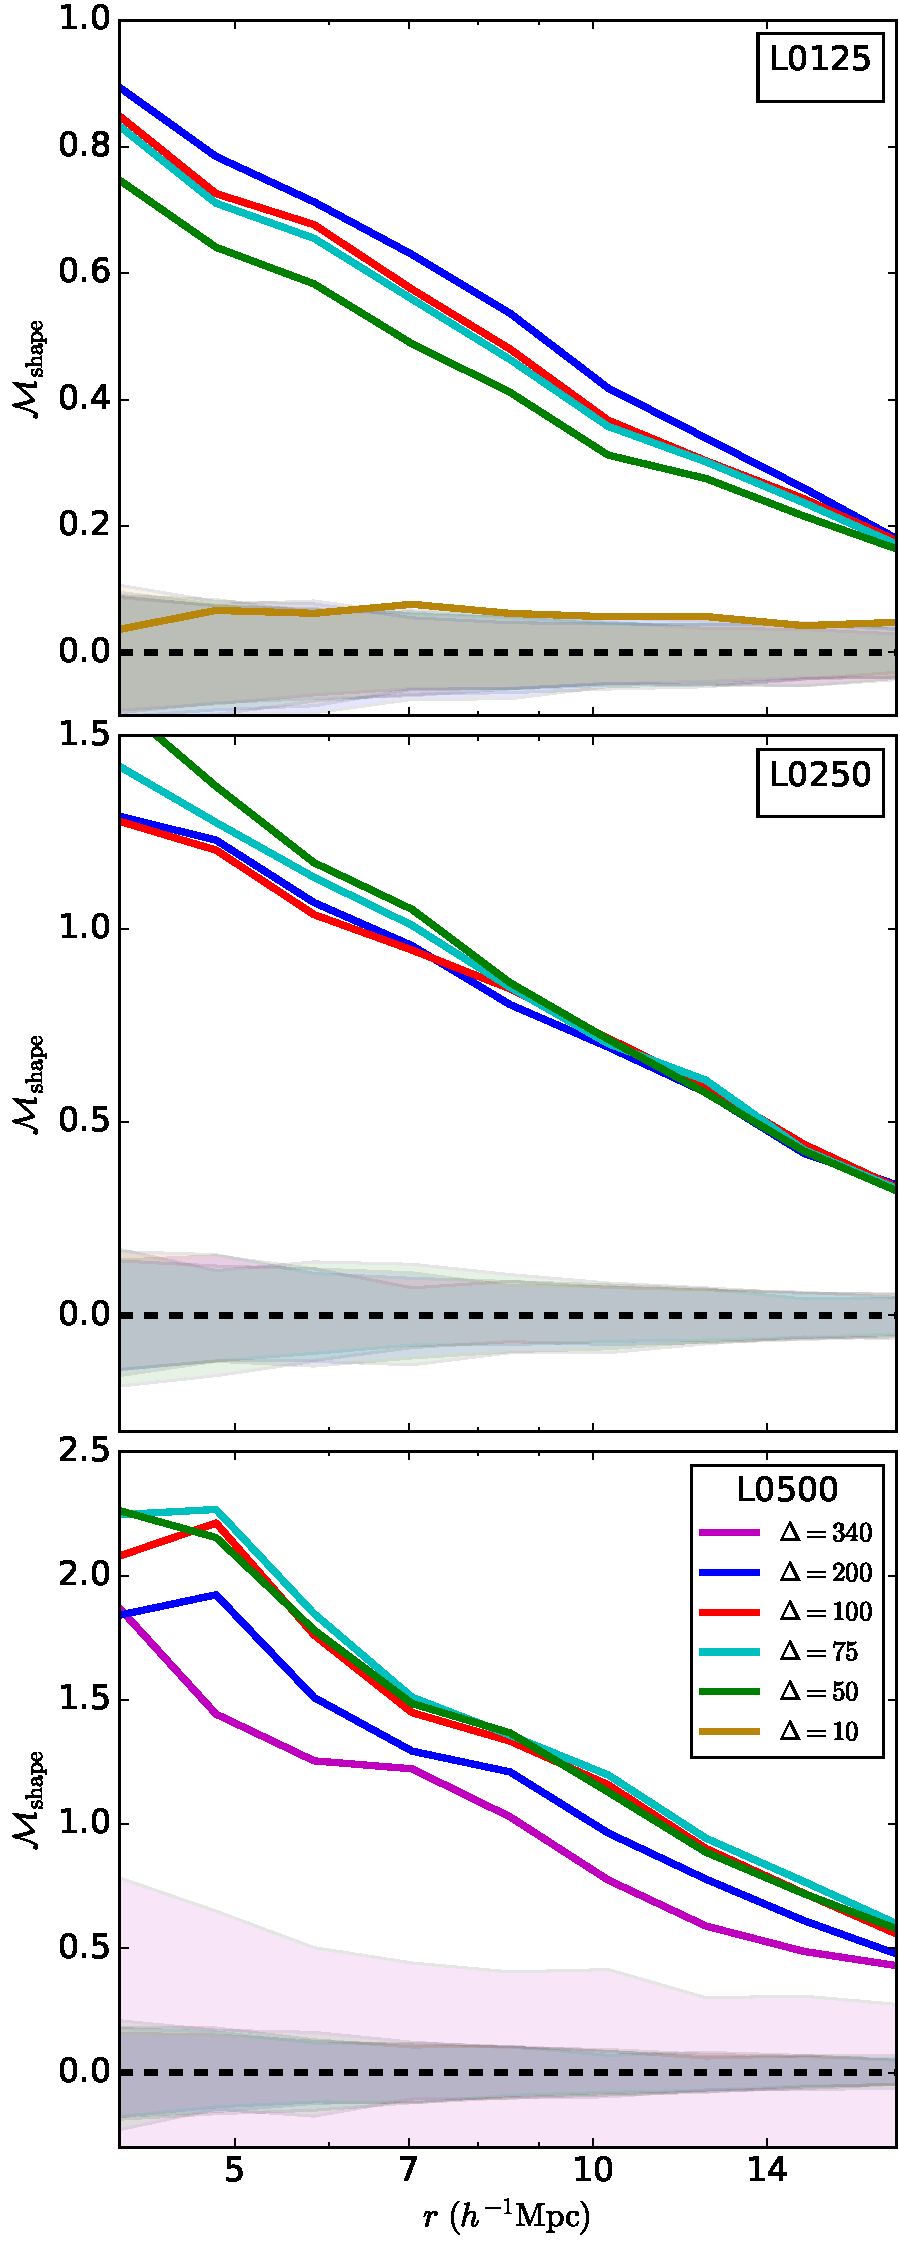
\includegraphics[width=.4\textwidth]{all_mcf_shape.pdf}
	\caption{
The marked correlation function for the halo shape parameter. In each plot the lines correspond to different values of $\Delta$, with dark blue (light blue) corresponding to $\Delta = 340$ ($\Delta = 50$). The red dashed line corresponds to the overdensity chosen for matching as possibly removing assembly bias on most scales in the case of halo concentration. The top (middle/bottom) panel shows the results for the
\simA \ (\simB /\simC) data set utilizing the low mass-shape (mid mass-shape/high mass-shape) cutoffs. The shaded bands represent 2-sigma confidence regions generated by randomization of the marks.}
	\label{fig:cc_mcf_s}
\end{figure}
%--------------------------------------------

\arz{A few comments here on the shape disussion and on Figure~\ref{fig:cc_mcf_s}. First, does your discussion really 
go with what is shown in the plot? I see that going down to 
$\Delta=20$ helps A LOT. Related to this, the red dashed lines 
in the middle and bottom panels don't make sense? They are clearly 
not the best case scenarios. In fact, it looks to me like the best 
case should be $\Delta=20$ in ALL PANELS! Am I missing something? Finally, you don't discuss Figure~11 AT ALL in the paper? Is it necesssary? I think probably not?}
\asv{Added in lines about how our red dashed lines are best case with regards to halo concentration. I also will remove the figure on how shape evolves with $\Delta$ - that was more relevant when we were getting shape measurements that were anomalous with previous paper results.}
Moving on from concentrations, Figure~\ref{fig:cc_mcf_s} illustrates MCFs in which the mark is the normalized rank of the shape parameter, $s$, of the halo. Similar trends as the previous cases repeat themselves in the case where shape is used at the trace mark. For the entire range of halo masses studied, the fiducial halo definition shows that more clustered halos have more spherical halos (e.g. halos with larger $s$ values). Furthermore, our change in halo definition shows that increasing the size of halos (and decreasing $\Delta$) leads to the most clustered halos having less spherical halos.

Where the environmental dependence associated with the shape parameter distinguishes itself is in finding the best fit value of $\Delta$ for removing the halo assembly bias. No reasonable value of $\Delta$ seems to be
capable of removing the enhanced clustering at the scales that we study, though the impact is reduced. We note that the best fit matches for concentration, the red-dashed lines in Figure~\ref{fig:cc_mcf_s}, do not correspond with removing assembly bias from shape. This failure may be driven by the filamentary nature of large-scale structure. Halos in overdense regions will gain mass as their halo radius expands that is not associated as substructure. If this additional mass accumulates with a preferred direction, as may be expected along a filament, this could induce a more elliptical halo shape. A detailed test of this hypothesis is beyond the scope of this paper, but may well be testable through association of halos with large-scale structure.

It should be noted that the process by which {\tt ROCKSTAR} calculates shape does inherently exclude substructure. Since subsumed host halos are identified as substructure in catalogs with lower values of $\Delta$, their mass is not included in the calculation of halo shapes. While beyond the scope of this work, it is possible that inclusion of substructure into our halo shape calculations could result in an improved reduction of assembly bias. This may merit future investigation.\asv{Or so I propose. I figure that this requires full particle data or a modification to {\tt ROCKSTAR}. It would be valuable to do, but would delay the paper more than I care to sort out in the meantime. That being said, if it does work for spin, it would be important to know about.}

%------------------
\subsubsection{Halo Spin}

\arz{Spin-dependent clustering does NOT give qualitatively the 
same results as shape-dependent clustering. This paragraph needs 
to be re-written. And again, in Fig.~\ref{fig:cc_mcf_spin}, the red dashed lines do not make sense to me. They are clearly NOT the best choices for the case of spin.}\asv{Some incorrect holdovers here. Fixing now.}
The spin MCFs are shown in Figure~\ref{fig:cc_mcf_spin}. Halos that are more clustered show higher values of the spin mark than would be expected from a uniform distribution of ranks. As with halo shape, it can be seen that the best match for halo concentration (the red-dashed lines in Figure~\ref{fig:cc_mcf_spin}) are poor fits for removing assembly bias from halo spin.\arz{Search the literature, particularly Brandon Allgood's papers and Andreas Faltenbacher whose 
names come to mind, for spin-dependent assembly bias. I'm trying to figure out if yours is the first paper 
to point this out.}\asv{Need to track down all the specific citations, but after changing our normalization
method, it seems to match up better with existing texts.}
\arz{Citations here still need to be done.} However, halo spin shows a qualitative response to our methodology which is opposite from previous results. Increasing halo radii by decreasing $\Delta$ only serves to increase the impact of assembly bias in this case; effectively our newly defined halos have higher spins than average in this case. As with halo shape, one can invoke a model relating back to filamentary structure. If new material is accumulated along some preferred direction, it is not unreasonable to conclude an increased value of spin. This might enhance the impact of assembly bias as a result of our method.


%---------------- spin MCF
\begin{figure}
	\centering
	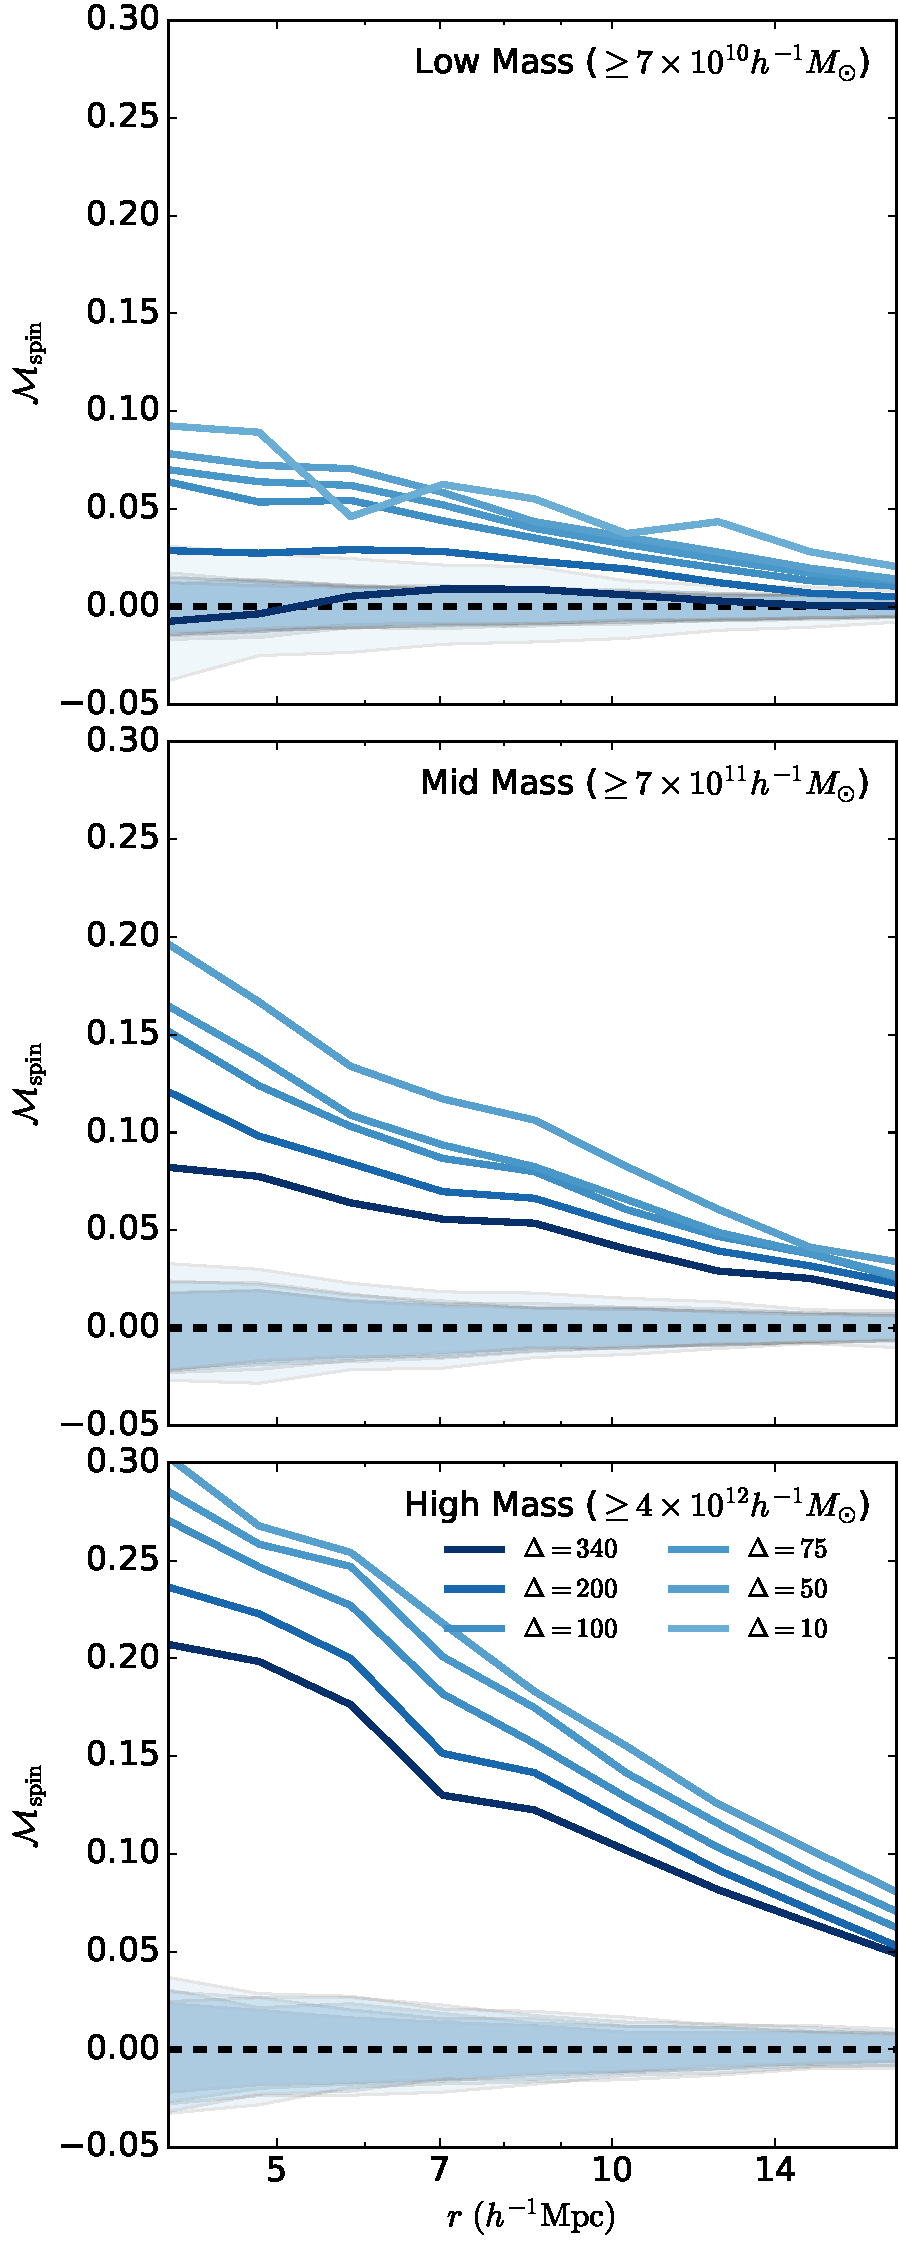
\includegraphics[width=.4\textwidth]{all_mcf_spin.pdf}
	\caption{
The marked correlation function for the halo spin parameter. 
The solid lines plot the marked correlation function using halo spin as the mark. In each plot the lines correspond to different values of $\Delta$, with dark blue (light blue) corresponding to $\Delta = 340$ ($\Delta = 50$). The red dashed line corresponds to the overdensity chosen for matching as possibly removing assembly bias on most scales for halo concentration. The top (middle/bottom) panel shows the results for the
\simA \ (\simB /\simC) data set utilizing the low mass (mid mass/high mass) cutoffs. The shaded bands represent 2-sigma confidence regions generated by randomization of the marks.
	}
	\label{fig:cc_mcf_spin}
\end{figure}
%-------------------------------

\subsubsection{Subhalo Abundance}

%----------------- satellite number MCF
\begin{figure}
	\centering
	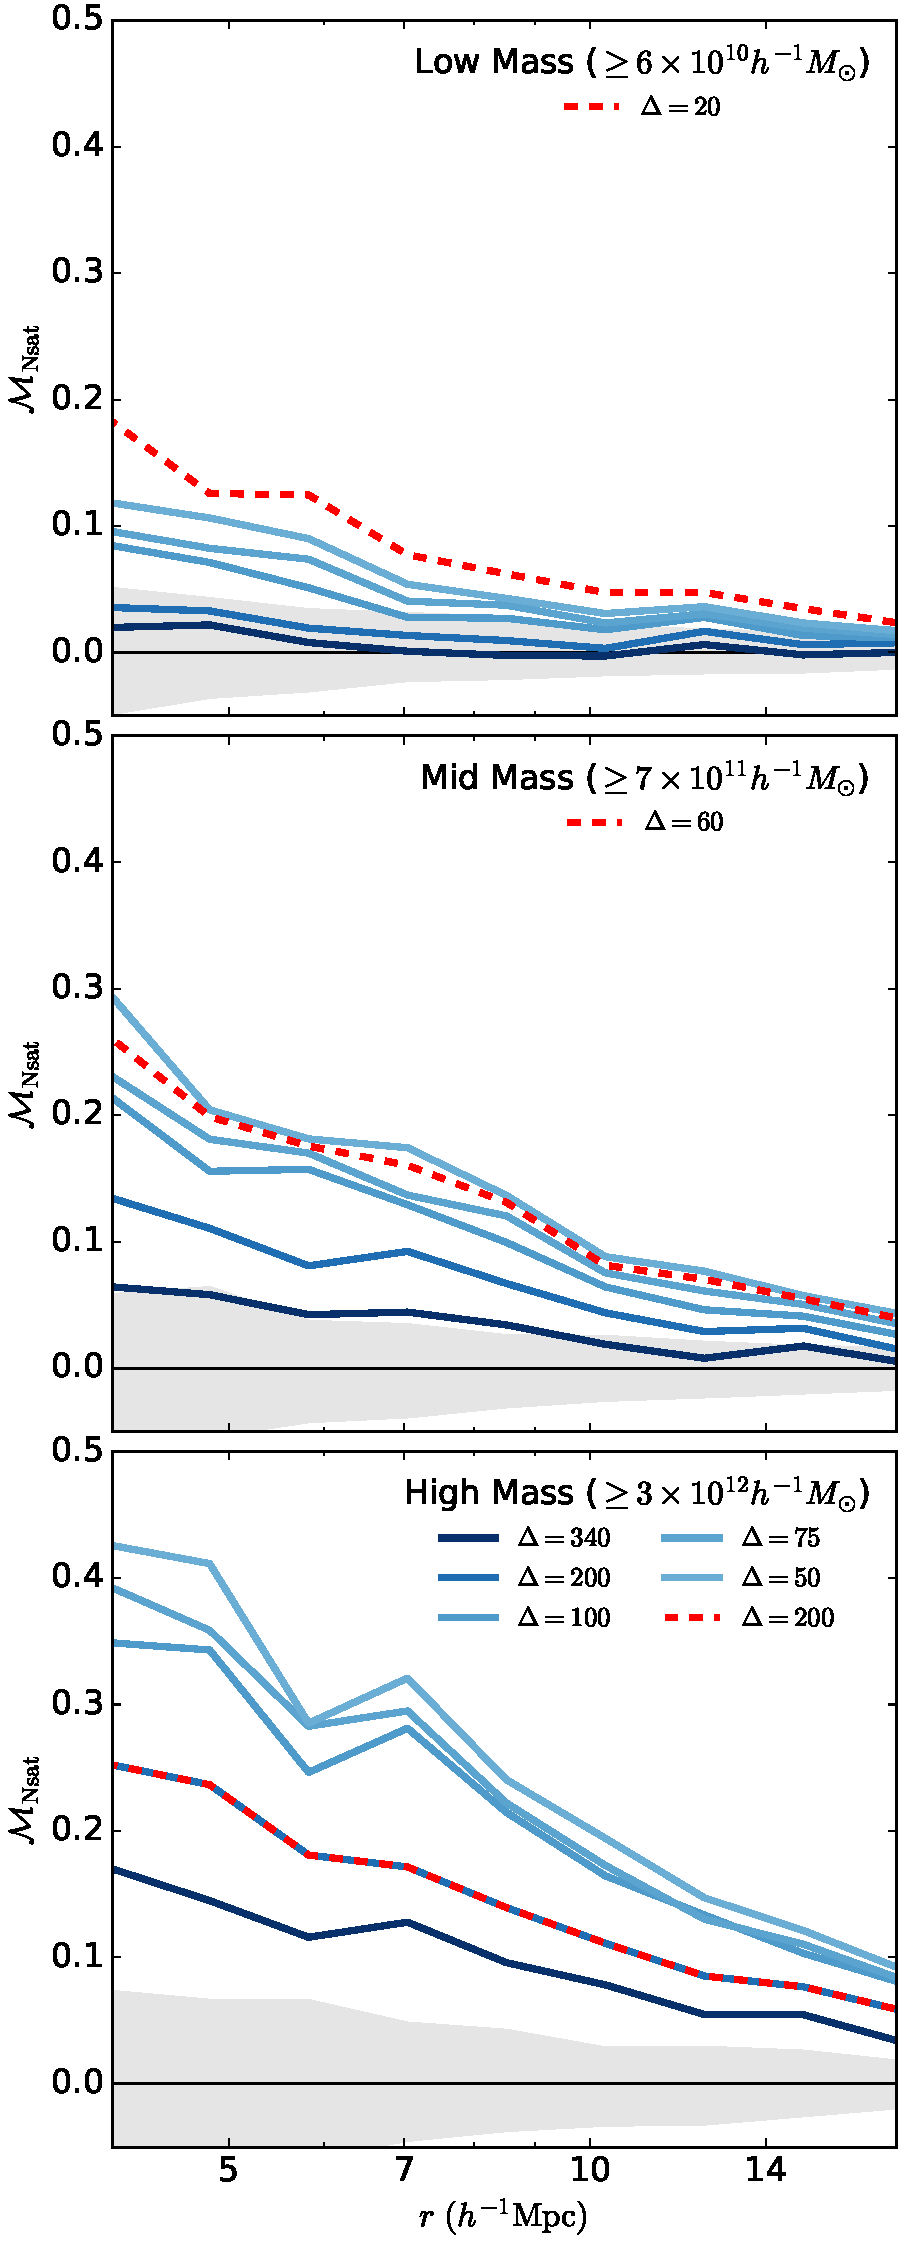
\includegraphics[width=.4\textwidth]{all_mcf_nsat.pdf}
	\caption{
The marked correlation function for the satellite number parameter. The solid lines plot the marked correlation function using halo satellite number as the mark. In each plot the lines correspond to different values of $\Delta$, with dark blue (light blue) corresponding to $\Delta = 340$ ($\Delta = 50$). The red dashed line corresponds to the overdensity chosen for matching as possibly removing assembly bias on most scales for halo concentration. The top (middle/bottom) panel shows the results for the
\simA \ (\simB /\simC) data set utilizing the low mass (mid mass/high mass) cutoffs. The shaded bands represent 2-sigma confidence regions generated by randomization of the marks.}
	\label{fig:cc_mcf_nsat}
\end{figure}
%-------------------------------------------------------------------------------------------


The clustering of halos as a function of the number of satellite galaxies at fixed mass is of 
particular practical interest. Efforts to model survey data on the large-scale galaxy distribution, 
such as the halo occupation distribution (HOD) or conditional luminosity function (CLF) formalisms 
typically make the assumption that the multiplicity of satellite galaxies within a host dark matter 
halo depends solely upon halo mass. If this assumption is violated, then the phenomenological 
modeling of galaxy clustering can be more complicated than in these simplest scenarios.

\arz{Same comments here as with spin and shape. Red dashed lines are clearly not the best choices. I don't know what you are trying to illustrate with them?}\asv{Changes made to the caption and mention in the text.}
Figure~\ref{fig:cc_mcf_nsat} shows clustering marked by satellite number as described in 
\S~\ref{section:methodology}. For all values of $\Delta$, halo clustering is strongly dependent 
upon satellite occupation at all masses. We note that as we move to higher masses, the most clustered halos have higher satellite occupations. Once again we note that the halo definition that removes assembly bias from halo concentration does not serve as a good definition for satellite occupation. As with halo spin, defining halos to have larger radii (smaller 
$\Delta$) generally makes the environmental dependence of halo clustering more 
significant. Of course, our results pertain to satellite halos, or subhalos, rather than 
satellite galaxies, so the connection to observations and how one might 
model observed galaxy clustering is indirect, yet suggestive. We also note that the fact that the clustering
appears reduced at lower masses is qualitatively in agreement with the predictions from \citet{wechsler_etal06}. 


%---------------------------------------------------------------------------------------------
\section{Discussion}
\label{section:discussion}
%---------------------------------------------------------------------------------------------

%----------------------------
\subsection{General}
%----------------------------

We have studied the clustering of dark matter halos as a function of halo properties other than mass. We have confirmed that for conventional halo definitions halo clustering strength is a strong function of the  ``auxiliary properties" that we studied, namely halo concentration (either measured through a fit to the NFW profile or assigned non-parametrically as the ratio of the maximum circular velocity to
the virial velocity), halo shape, halo spin, and substructure content. These findings are consistent with the now significant literature on the subject subject of halo assembly bias. \citep{peacock_smith00, wechsler_etal02,sheth_tormen04, gao_etal05, zentner_etal05, allgood_etal06, harker_etal06, wechsler_etal06, croton_etal07, zentner07, dalal_etal08, zentner_etal14, mao_etal15, sunayama_etal16}

We have explored auxiliary property dependent halo clustering as a function of halo definition, parameterized by overdensity parameter $\Delta$. This exploration was motivated, in part, to determine whether 
alternative halo definitions can mitigate the dependence of halo clustering on these ``auxiliary properties." In general, we find that these alternative definitions do {\em not} significantly mitigate the effects of assembly bias. Moreover, these modified halo definitions, with low values of $\Delta$, often lead to stronger assembly bias, rather than weaker assembly bias. Concentration-dependent clustering is an exception to this conclusion that we will discuss further below.

An interesting and general conclustion that follow from our work is that auxiliary property dependent halo clustering, or assembly bias, depends greatly on halo definition. In each of Figures \ref{fig:cc_mcf_cnfw} through \ref{fig:cc_mcf_nsat}, the strength of assembly bias is a strong function of halo definition. This definition dependence is not restricted to extreme choices of the overdensity parameter $\Delta$. The difference in the strength of assembly bias between a ``virial'' halo definition, with $\Delta=340$, and a definition with $\Delta=200$ is considerable. Indeed, the difference can even lead to a difference in the {\em sense} of the assembly bias; higher concentration halos may be more strongly clustered by one halo definition and more weakly clustered by another. It is interesting to consider that differences on the strength of assembly bias in the literature may be partly induced by the different halo definitions used by different authors.

%------------------------------
\subsection{Mitigating Concentration-Dependent Clustering with Halo Definition}
%------------------------------

Our results suggest that halo redefinition may be able to mitigate concentration dependent halo clustering. This is evident in Fig.~\ref{fig:cc_mcf_cnfw} and Fig.~\ref{fig:cc_mcf_cV}. Halo concentration is strongly correlated with halo formation time, so this suggests that such a redefinition {\em may} aid in reducing assembly bias associated with halo formation time; however, this is a non-trivial extrapolation of our results and a follow-up study to assess halo formation times in alternative halo definitions is both interesting and warranted. 

Clearly, the halo definition that best mitigates concentration-dependent assembly bias must be mass dependent. Low values of $\Delta$ ($\Delta \sim 25$ with $R_{25} \sim 2R_{200}$) seem appropriate near for our lowest mass-threshold sample (with $M_{200} \ge 7 \times 10^{10} \hMsun$) whereas $\Delta \sim 200$ or slightly higher is adequate for our highest mass threshold sample (with $M_{200} \ge 4 \times 10^{12} \hMsun$). 

This result is reminiscent of much recent work on the so-called halo ``splashback radius" \citep{more_etal15} and, indeed, our efforts were partly motivated by this work. We note that while the splashback radius methodology does seem similar in concept to our methodology, Fig. ~\ref{fig:splashback_compare} demonstrates that a one-to-one comparison between the two methods is difficult
at best. While both our method of halo redefinition and their determination of splashback radius seem to show a
monotonic trend in mass, we note that our work with the lowest mass halos requires a definition of halo radius
that substantially larger than the splashback radius method alone might suggest.


\begin{figure}
	\centering
	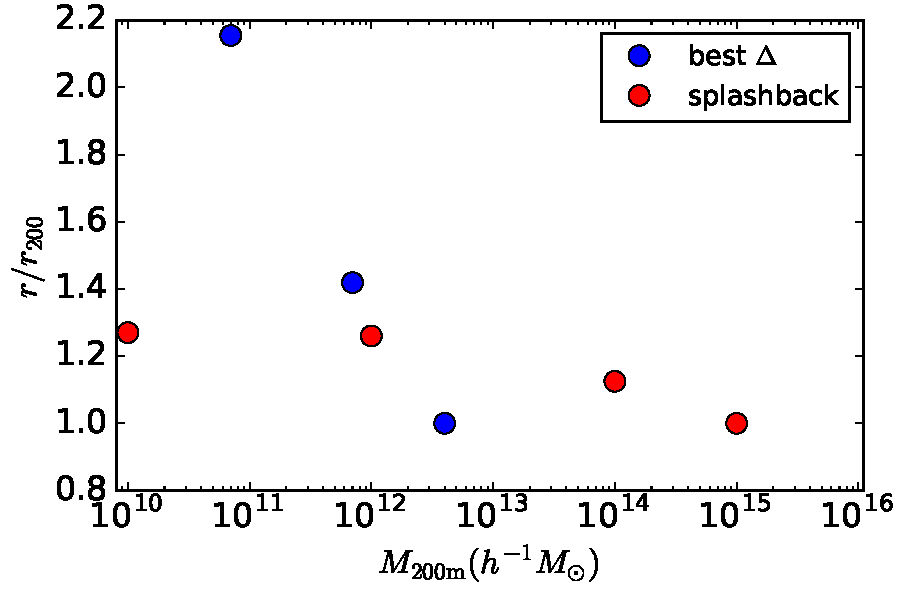
\includegraphics[width=.4\textwidth]{test_splashback.pdf}
	\caption{A comparison of the average ratio between $r_{200}$ and the splashback radius as determined by
	 \citet{more_etal15} (red circles) to the average ratio between $r_{200}$ and the halo radius determined as our
	  best fit for removal of assembly bias as discussed above (blue circles). Note that the halo mass chosen for
	  the blue points is determined by the mass cutoff in the simulation analysis, as the smallest (and most
	  numerous) halos dominate the calculation.}
	\label{fig:splashback_compare}
\end{figure}


It is useful to investigate the reasons why halo redefinitions may be helpful in the case 
of concentrations. On the positive side, it is possible that these redefinitions do define 
halos an a more practically useful way, better isolating objects that have been strongly 
altered by nonlinear evolution from the larger-scale environment. In this case, halo redefinition 
would be a step forward. However, it is also possible that the details of measuring halo 
properties using these new halo definitions introduce new sources of noise into the 
measurements. If this is the case, then the reduction in environmental effects stems 
from the fact that them measurement of the halo property 
introduces noise and is {\em less} informative about the halo itself. 
For the case of halo concentration, which is the most interesting to 
follow up, introducing noise can happen in numerous ways. For example, 
the NFW concentration $c_{\mathrm{NFW}}$ is determined by a fit to the 
NFW profile. Inferred values of $c_{\mathrm{NFW}}$ will depend upon 
the degree to which the density profiles of the halos follow the NFW 
functional form within some radius $R_{\Delta}$ that is different from 
traditional halo radii, such as $\sim R_{200}$. At large halocentric 
distances ($r \gtrsim R_{200}$) halo profiles are known to deviate 
from the NFW form. It is worth noting that the velocity-defined concentration 
$c_{\rm V}$ is a non-parametric measure of concentration and should be 
less subject to such effects. 

We note that the mean dispersion of halo concentrations for a given mass
bin are not significantly changed as we move to our best fit value of
overdensity parameter, $\Delta$. This is highly suggestive of the fact
that the success of our method is not the result of larger measurement
error, but is more fundamental to the nature of relating halo definition to
our halo parameters of interest.\arz{Now you mention the interesting part about the new figure. 
This should be a discussion of how much larger/smaller the dispersion in 
concentrations gets for, say $\Delta=70$ compared to $\Delta=200$.}
\asv{The dispersion of halo concentrations is not significantly changed -
while a little smaller, it is well within the scatter of the dispersion as
well.}

We can explore in more detail the degree to which the mitigation of environmental 
effects by halo redefinition are due to introducing noise that is uncorrelated with 
environment into the measurement of halo properties when halos are defined 
in a manner distinct from the more traditional definitions. We proceed as follows. 
All host halos that are found in the halo catalogs constructed from lower values 
of $\Delta$ (for example, $\Delta ~ 60$ which is an interesting value for exploring 
concentration in the mid-mass cut of the L0250 simulation) are present as host halos in the halo 
catalogs constructed with higher values of threshold density (e.g., $\Delta = 200$). 
We match each halo in the lower threshold (lower $\Delta$) simulation to 
its corresponding halo in the higher threshold catalog. We then consider 
the clustering of only those halos that we have matched across catalogs. 
We refer to these as the ``matched" halo samples between two values 
of threshold overdensity $\Delta$. 


\begin{figure}
	\centering
	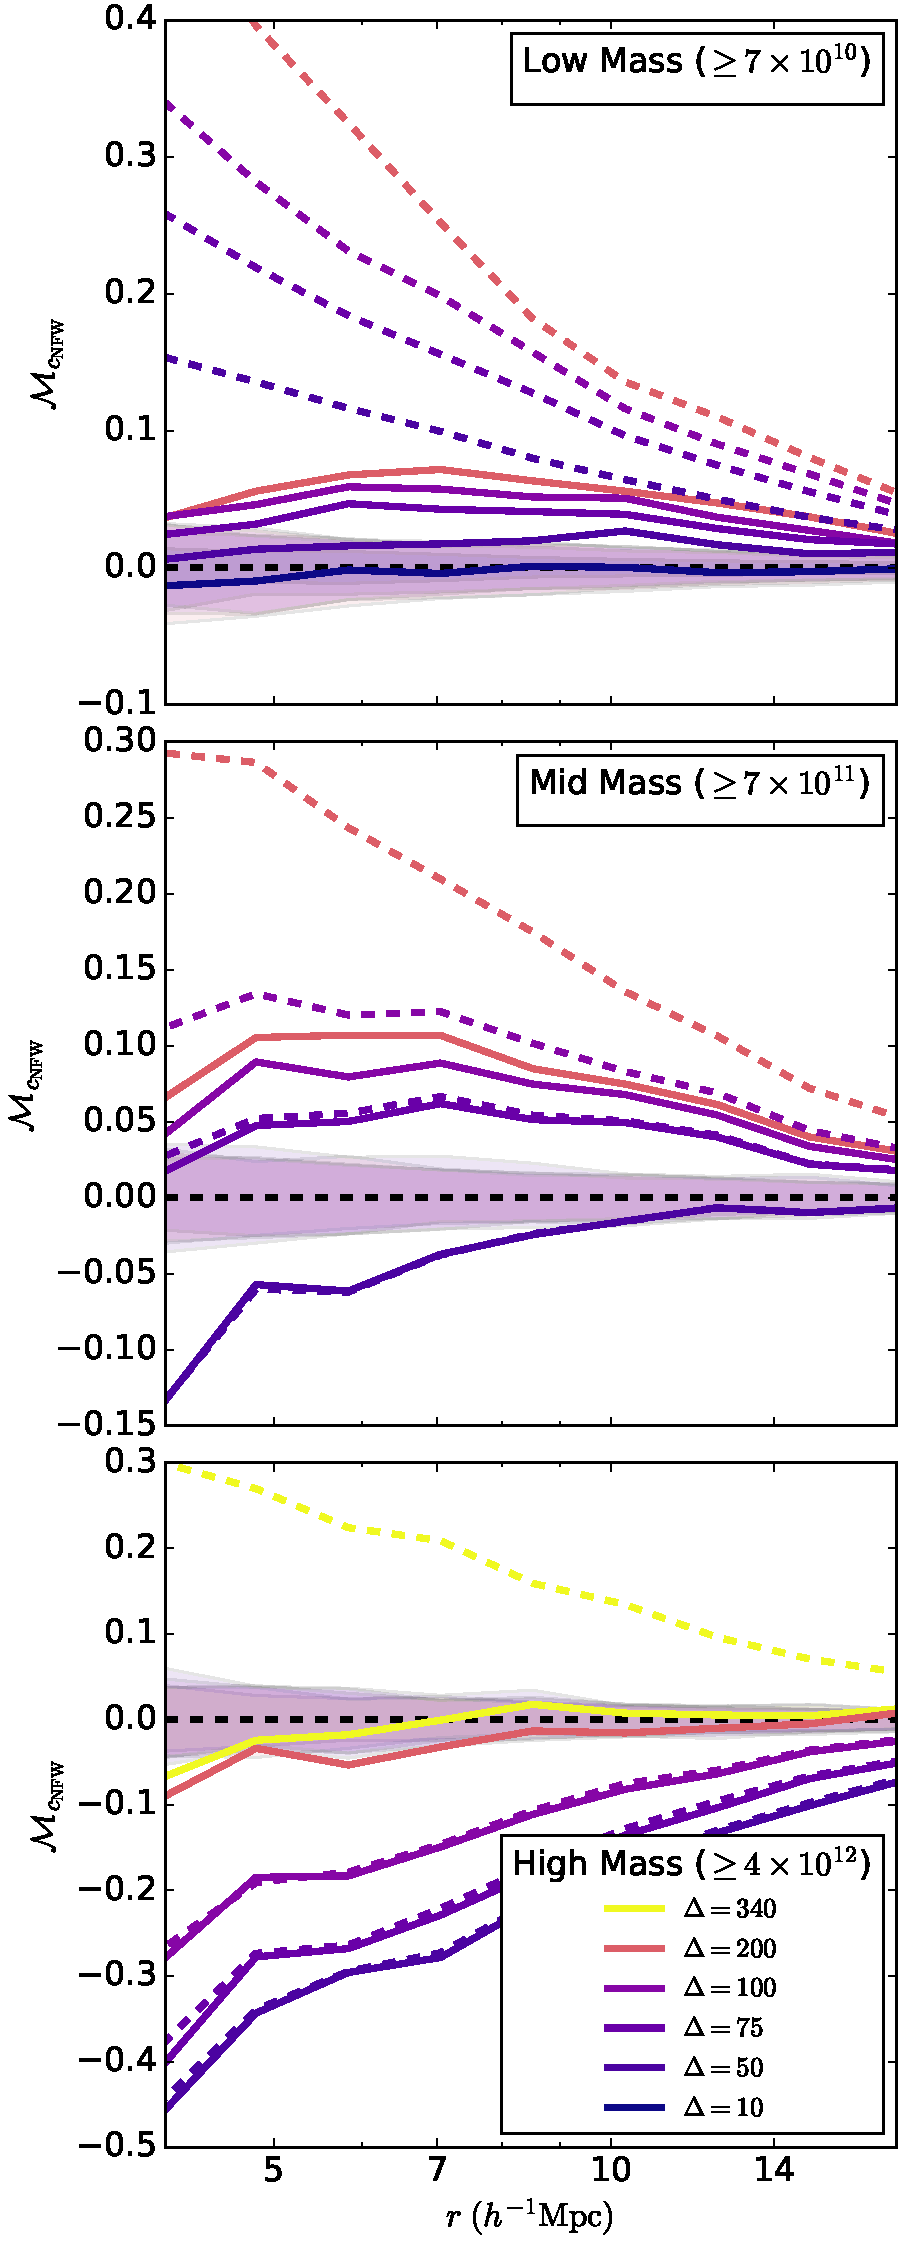
\includegraphics[width=.4\textwidth]{match_mcf_cNFW.pdf}
	\caption{The marked correlation function for the NFW-defined halo concentration parameter. The solid lines plot the marked correlation function using NFW-defined halo concentration as the mark, for a catalog matched against the best fit $\Delta$ shown in red. The dashed lines plot the original marked correlation function results. In each plot the lines correspond to different values of $\Delta$, with dark blue (light blue) corresponding to $\Delta = 340$ ($\Delta = 50$). The red dashed line corresponds to the overdensity chosen for matching as possibly removing assembly bias on most scales for halo concentration. The top (middle/bottom) panel shows the results for the
\simA \ (\simB /\simC) data set utilizing the low mass (mid mass/high mass) cutoffs. The shaded bands represent 2-sigma confidence regions generated by randomization of the marks. Only host halos consistent with the best-fit catalog from above are included in the analysis.}
	\label{fig:hvm_mcf_cnfw}
\end{figure}

\arz{Please check to ensure that I know what you mean by your matched samples. Your language was not 
specific enough for me to be 100\% sure. Modify as necessary.}
\asv{Looks absolutely correct to me.}
Figure~\ref{fig:hvm_mcf_cnfw} shows the same statistic as Figure~\ref{fig:cc_mcf_cnfw}, except for matched
subsamples. The matched subsamples are matched to a catalog generated for the value of $\Delta$ most likely to
remove assembly bias at large scales for the concentration marks; $\Delta=20$ for the `Low Mass' cut, $\Delta=60$,
for the `Mid Mass' cut, and $\Delta=200$ for the `High Mass' cut. These matched halo catalogs only differ from
the standard halo samples in that they contain only those host halos common 
to both the catalog in question and the best fit $\Delta$ catalog. One particularly interesting result is noted in the \simB~ data. First draw your attention to the
difference between the unmatched (dashed lines) and matched (solid lines) catalog results; this change is driven entirely by the exclusion of host halos due to a change in halo definition, as all other properties are consistent between catalogs. This is highly suggestive that most of the assembly bias signal is driven by the interaction of host halos with other nearby halos. The remaining component of the reduction of assembly bias signal is driven by an increase in noise or some more fundamental difference in how the marks are measured or mass is assigned. We look forward to probing the impact of these effects in the future.

From Fig.~\ref{fig:hvm_mcf_cnfw}, it is apparent that some degree of assembly bias persists in the matched 
samples. Yet, what is interesting is that a very significant fraction of the assembly bias effect has been 
removed compared to the standard $\Delta=200$ result. The halos in the matched catalogs have the 
same properties (including $c_{\mathrm{NFW}}$) as those in the standard catalogs, so that removal 
of assembly bias is {\em not} due to introducing noise or other systematics into the measurement of 
concentration. That mitigation of assembly bias is due to the halo redefinition and, in particular, 
subsuming those halos most subject to assembly bias effects as subhalos of the $\Delta=70$ 
halos. This is an interesting result suggesting that seeking optimal halo definitions may be 
one avenue to more completely separating the strongly nonlinear evolution occurring within 
halos from large-scale evolution and mitigating assembly bias. 


\begin{figure}
	\centering
	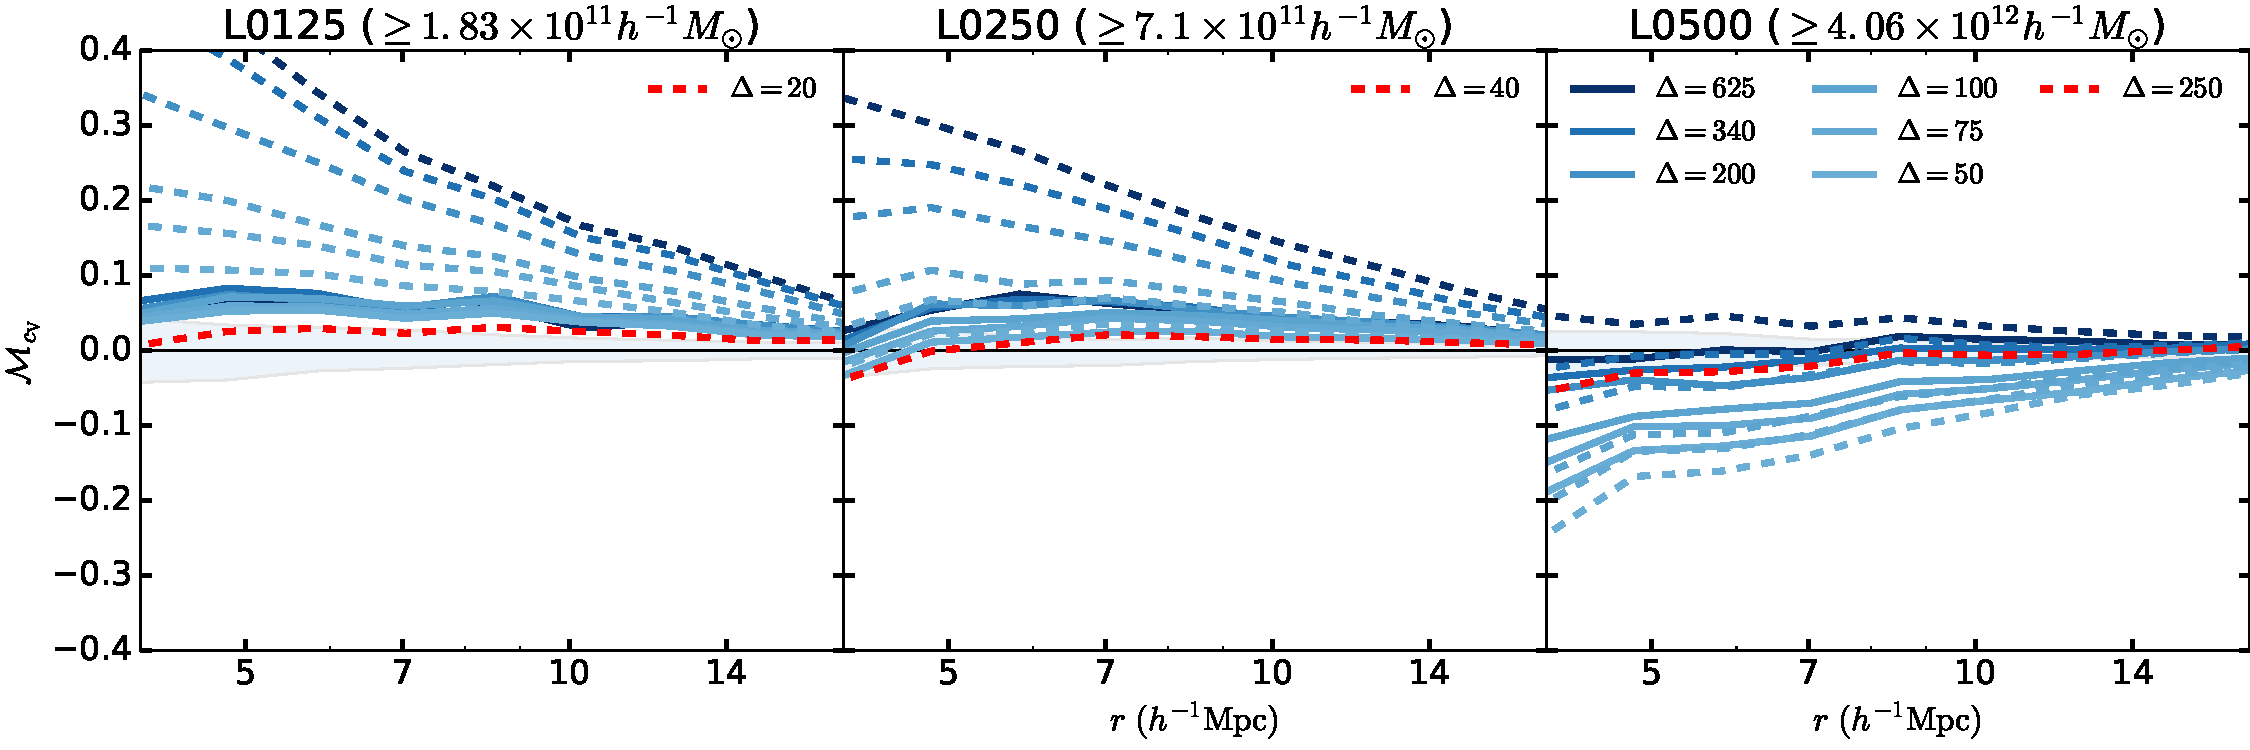
\includegraphics[width=.4\textwidth]{match_mcf_cV.pdf}
	\caption{The marked correlation function for the velocity ratio defined halo concentration parameter. The solid lines plot the marked correlation function using velocity ratio halo concentration as the mark, for a catalog matched against the best fit $\Delta$ shown in red. The dashed lines plot the original marked correlation function results. In each plot the lines correspond to different values of $\Delta$, with dark blue (light blue) corresponding to $\Delta = 340$ ($\Delta = 50$). The red dashed line corresponds to the overdensity chosen for matching as possibly removing assembly bias on most scales for halo concentration. The top (middle/bottom) panel shows the results for the
\simA \ (\simB /\simC) data set utilizing the low mass (mid mass/high mass) cutoffs. The shaded bands represent 2-sigma confidence regions generated by randomization of the marks.}
	\label{fig:hvm_mcf_cV}
\end{figure}

\arz{Put a discussion of Fig.~\ref{fig:hvm_mcf_cV} here. It does not need to reiterate the discussion of 
Fig.~\ref{fig:hvm_mcf_cnfw}. However, it should state that we reach the same broad conclusion and that 
this is good in part because $c_{\mathrm{V}}$ is a nonparametric measure of halo concentration.}
Figure~\ref{fig:hvm_mcf_cV} follows the same exercise as above, with a comparison drawn to the Fig.~\ref{fig:cc_mcf_cV}. Notice that the same trends as Fig.~\ref{fig:hvm_mcf_cnfw} can be seen: a significant fraction of assembly bias is removed as compared to the unmatched catalog, though statistically significant assembly bias remains. Only in combination with halo redefinition do we remove assembly more completely on large scales. Note that the max circular velocity defined concentration is nonparametric by design; this helps to confirm that our result is not related to choice of halo density profile.

\arz{This paragraph is good, but needs to be written a bit more professionally. Start with a sentence like, 
``It is interesting to explore the reasons that halo shape, spin, and satellite number are not amenable 
to having their assembly bias mitigated through simple halo redefinitions." Then move on to some specifics.}
\asv{attempted to rewrite more professionally!}

While halo shape, spin, and satellite number are not amenable to having their assembly bias mitigated through the
simple halo redefinition technique we have suggested, the underlying reasons for this behavior remains of
interest for exploration. In the case of halo shape, we suggest that the assembly bias may be driven through
interactions with large scale structure. Studies have shown a statistically significant alignment between
filaments and satellite galaxy position \citep{tempel_etal15, velliscig_etal15}\asv{need to grab paper from arxiv
2016.05.09 for this}.

Note that the mass dependence of assembly bias is implicitly explored with our suite of simulations.
The nature of the MCFs emphasizes halos just above the threshold mass; e.g. \simA~ probes the smallest mass
halos, while \simB~ probes the largest mass halos. To more explicitly explore this mass dependence, Figure~\ref{fig:biascompare}
demonstrates how bias scales as a function of both fixed halo mass and choice of overdensity $\Delta$. Here we calculate the bias as follows:
\beq
b^2(r) = \xi_{c_\mathrm{NFW}} / \xi_{\mathrm{all}},
\eeq
where $\xi_{c_\mathrm{NFW}}$ consists of those halos with the 20\% highest marks in NFW-defined concentration
and $\xi_{\mathrm{all}}$ consists of all halos. Note that due to the limited number of halos in each mass bin, we choose not to use the binning and rank weighting that is utilized in previous analysis. \asv{This is currently how it is run and I am not sure if this is the best approach. We could probably afford to use ~5 bins and it would be a little more fine than when we carry out the full analysis.} To explore the mass dependency of the bias, we choose to
examine a fixed scale of 5 to 10 $\hMpc$. We calculate the bias using halos in bins of fixed mass, with errors
calculated using resampling in which $\xi_{\mathrm{all}}$ is replaced with the correlation function calculated
using a randomly chosen subsample of equal number to the biased subsample. The displayed error bars represent
the region in which 68\% of these random subsamples lie. We explore our dataset with the following binning,
in which the larger simulations are able to push to higher masses than the smallest simulation:
$7\times10^{10}-2\times10^{10}, 2\times10^{10}-7\times10^{11},7\times10^{11}-2\times10^{12},
2\times10^{12}-7\times10^{12},7\times10^{12}-2\times10^{13},2\times10^{13}-7\times10^{13},
7\times10^{13}-2\times10^{14} \hMsun$.

There are two clear trends to be determined from this data. The first is the trend for the assembly bias with
halo concentration to be reduced as a function of halo mass. This trend helps to resolve the apparent
inconsistencies in measures of assembly bias in the literature; namely, a change in halo mass of
interest can lead to a considerably different measure of halo assembly bias - at high masses, halo assembly
bias due to NFW-defined concentration is fairly minimal. The second visible trend is that a change in halo
definition chosen has a trend of decreasing the halo bias determined. Furthermore, it should be noted that this
can lead to an anticlustering of halos of high concentration at high masses. These two discoveries seem to
suggest that halo assembly bias of NFW-defined halo concentration is a coincidence; choosing a halo size
across all halo masses as a function of an overdensity will be insufficient in creating self-similiar dark
matter halos.
\arz{Instead, add one summarizing paragraph here discussing the mass dependence of assembly bias. 
Emphasize that our findings suggest that the strength of assembly bias can be a strong function of halo 
definition and that this may already be making it difficult to compare the results of various different research 
groups using different halo definitions.}

\begin{figure*}
	\centering
	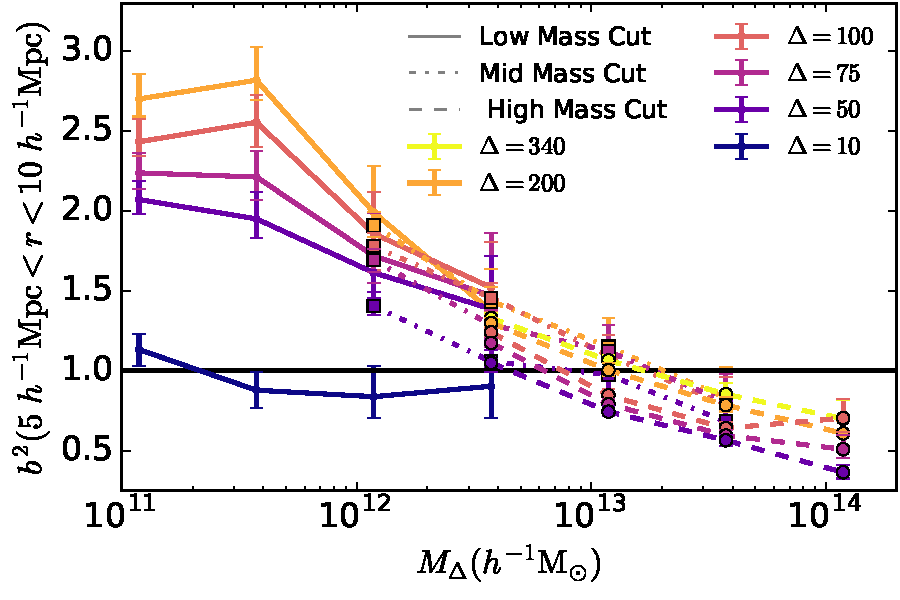
\includegraphics[width=.8\textwidth]{biasplot.pdf}
	\caption{
	The bias of the 20\% highest concentration sample to the full sample, plotted against halo mass measured at the halo radius. The halo mass binning is defined in full detail in the text. Halo definitions descend from the largest definition to lowest definition, from dark to light in color. The dark blue (light blue) line uses a halo definition drawn from $\Delta = 340$ ($\Delta = 50$). The solid (dot-dashed, dashsed) lines use host halos from the \simA (\simB,\simC) catalogs. The
	error bars encompass 68\% of measurements using two hundred subsamples
	of the mark of the same size as the biased sample. The solid black line
	shows where there is no detected assembly bias driven by NFW-defined halo concentration.}
	\label{fig:biascompare}
\end{figure*}


%----------------------
\section[]{Conclusions}
\label{section:conclusions}
%----------------------

\arz{After dealing with the comments above, let's come back to rewriting the conclusions section.}
We have looked at how to use CFs and MCFs in order to analyze the environmental effects upon the properties of the halo. We have suggested a method of removing the mass dependence that is not subject to the small number statistics at large halo masses. Taking our various tests, we then apply a change to the threshold density $\Delta$ in an attempt to remove the effect that environment has upon these properties. We come to the following conclusions from our simulation data.

\begin{itemize}
	\item Our halo redefinition method does not cause any substantial breakdown in the ROCKSTAR halo finding
algorithm, though this may not be the case for every halo finding methodology. This is something that should be
considered prior to utilization of this method, unless working directly from particle data. As our initial halo
sizes and locations are determined through spherical overdensities, it cannot be assumed that starting from a FoF
grouping and then determining values through particle data directly will produce identical results. Similarly,
different cosmologies may remove environmental effects at different scales.

	\item When looking at the two-point correlation function, there appears to be a ``sweet spot'' that appears
to remove environmental effects the most efficiently. Going beyond that seems to reintroduce environmental
effects, possibly as an extreme side effect of halo exclusion.

	\item For our marked correlation functions we see that both proxies of concentration that we use as marks
show significant removal of environmental effects at large scales for similar values of the overdensity parameter
$\Delta$. In cases where one is only interested in the concentration of dark matter halos and large scales (or
correspondingly small values of k), this method will allow you to compensate for bias that environment could
introduce to calculations dependent upon the halo model. This may prove valuable for calculations such as that of
the shear power spectrum calculated through weak lensing.

	\item The environmental effects on the shape of the host halo and the satellite number of the host halo
cannot be removed regardless of the chosen redefinition of $\Delta$. We propose that this may be intrinsically
tied to the nature of the filaments, whose effects cannot be removed by a simple redefinition of the halo radius.

	\item This method is definitively related to the mass of the halos that are being observed. Furthermore, it
appears that the majority of the reduction in assembly bias is tied to the exclusion of halos from the catalog as
a result of being subsumed into larger halos. This information does not seem to be contradictory; it can be
intuitively understood that the region about the most massive halos will be different than the region around the
least massive halos, leading to a different frequency at which halos are being excluded. It does however warrant
that careful consideration be given to the sample of halos that are of interest.

	\item The selection of halo size is intrinsically related to the assembly bias and varies across scales. This
might help to resolve contradictory results in the search for halo assembly bias in the literature.
\end{itemize}

This methodology, while certainly not perfect in accounting for assembly bias, may be of significance when
applied to galaxy formation models and give insight into seemingly conflicting results. Provided that the
properties of interest in a given model behave well under our redefinition, it will allow us to create better
mock galaxy catalogs without resorting to more complicated models requiring halo formation histories - giving us
another powerful tool to test observation against.

There remain possible uncertainties to study in the future. One possible area of follow-up is the matter of
simulation cosmology, which is not explored in this text. It is possible that the choice of cosmology may change
observed assembly bias as a function of the halo masses, something that our methodology should be capable of
observing. Furthermore, we can determine if the choice of halo size that best reduces assembly bias is a function
of the chosen cosmology. This may be of interest in attempting to determine signatures of assembly bias in
observational samples in the future.

\section*{Acknowledgments}

We are grateful to many people. Our calculations are carried out utilizing the
{\tt numpy} \citep{numpy}, {\tt astropy} \citep{astropy}, {\tt matplotlib} 
\citep{matplotlib}, and {\tt halotools} \citep{halotools} packages in Python.

%%\bibliographystyle{plainnat}
\bibliography{master}

\section*{Appendix}
\label{section:appendix_massres}

One natural question that might arise in the analysis of this work is the nature of the resulting assembly bias
trends. Our focus in the main sections of this paper is on the nature of the assembly bias changing as a function
of the mass cut chosen. Our conclusions include the fact that there is a strong mass dependence on halo assembly
bias that must be accounted for separately depending on the halos of interest in a study. However, while the
existence of this trend is clear within our analysis, the determination that this is solely due to the masses of
the halos included in our calculation is less clear upon closer inspection. One possibility that might be
particularly concerning is the potential that the different simulations have created halos that have
fundamentally different clustering and this is leading to the result that we are interpreting as a mass
dependence on assembly bias. Thankfully, though our statistics become less meaningful to carry out this
calculation, we can carry out a comparison using the same mass cut across two of our simulations, knowing that
these will only contain well resolved halos.

While not addressed directly, Figure~\ref{fig:hvl_cfcompare} through Figure~\ref{fig:hvl_mcf_nsat} contain a
demonstration of the result that we are seeking in the left column of panels. The lower left panels show various
marks of interest for \simB \ using the ``mid mass'' cut on the data set. In comparison, the upper left panel
contains the same marks of interest for the \simA \ using the same mass cut. In the latter, there are fewer halos
in this mass cut range, as a result of the smaller simulation box size. However, we note that despite the
additional noise in the data set, the behavior of the assembly bias measurement is nearly identical within
tolerances accounting for differences between simulations and noise. This motivates our conclusion that the
driver behind the behavior is the mass cut of the data sets rather than the resolution of the simulation.

\label{lastpage}

\end{document}
